\documentclass[eng,printmode,openany]{mgr}
\usepackage[utf8]{inputenc}
\usepackage{polski}
\usepackage[polish]{babel}
\usepackage{graphicx}
\usepackage{subfigure}

\usepackage{psfrag}
\usepackage{amsmath}
\usepackage{amsfonts}

\usepackage{supertabular}
\usepackage{array}
\usepackage{tabularx}
\usepackage{hhline}
\usepackage{showlabels}
\usepackage{float}
\usepackage[square,sort,comma,numbers]{natbib}
\usepackage{multirow}

\usepackage{url}
\def\UrlBreaks{\do\/\do-}
\usepackage{breakurl}


\newcommand{\R}{I\!\!R}
\newtheorem{theorem}{Twierdzenie}[section]

\usepackage[toc,page]{appendix}

\usepackage{listings}
\usepackage{xcolor}
\colorlet{punct}{red!60!black}
\definecolor{background}{HTML}{EEEEEE}
\definecolor{delim}{RGB}{20,105,176}
\colorlet{numb}{magenta!60!black}

%\renewcommand{\bibname}{Literatura}
%\renewcommand\refname{Literatura}
\renewcommand\lstlistingname{Listing}
\renewcommand\lstlistlistingname{Spis listingów}

\lstset{
	basicstyle=\small,
	breaklines=true
}

\lstdefinelanguage{json}{
	string=[s]{"}{"},
	stringstyle=\color{blue},
	comment=[l]{:},
	commentstyle=\color{black},
}
% frontpage
\title{Aplikacja webowa wspomagająca zarządzanie flotą samochodów}
\engtitle{A web application supporting cars fleet management}
\author{Jan Pajdak}
\supervisor{dr inż. Jarosław Mierzwa, W4/K9}
%\guardian{dr hab. inż. Olgierd Unold Prof. nadzw. PWr, K-9}
\field{Informatyka (INF)}
\specialisation{Inżynieria systemów informatycznych (INS)}

\begin{document}
	\bibliographystyle{plainnat}
	\renewcommand{\bibname}{Literatura} 
	\renewcommand{\appendixtocname}{Dodatki}
	\appendixpageoff
	\maketitle
	%\dedication{6cm}{dedykacja \texttt{$\backslash$dedication}}
	
	\tableofcontents 
	

	\newpage	
	\addcontentsline{toc}{chapter}{\listfigurename}
	\listoffigures
	
	\newpage
	\addcontentsline{toc}{chapter}{\listtablename}
	\listoftables
	
	\newpage
	\addcontentsline{toc}{chapter}{\lstlistlistingname}
	\lstlistoflistings
	
	\chapter*{Skróty}
	\begin{itemize}
		\item \textbf{API} (ang. Application Programming Interface)
		\item \textbf{DB} (ang. Database)
		\item \textbf{GC} (ang. Garbage Collector)
		\item \textbf{UI} (ang. User Interface)
		\item \textbf{JSON} (ang. JavaScript Object Notation)
		\item \textbf{JWT} (ang. JSON Web Token)		
		\item \textbf{ORM} (ang. Object-Relational Mapping)
		\item \textbf{PK} (ang. Primary Key)
		\item \textbf{VS} (ang. Visual Studio)		
	\end{itemize}
	
	%----------------------------------------------------------------------------------------
	%	SECTION 0
	%----------------------------------------------------------------------------------------
	
	%----------------------------------------------------------------------------------------
	%	SECTION 1
	%----------------------------------------------------------------------------------------
	\newpage
	\chapter{Wstęp}
	\section{Wprowadzenie}
	Temat projektu został wybrany ze względu na chęć wykorzystania wiedzy z dziedziny motoryzacji w celu stworzenia aplikacji ułatwiającej zarządzanie pojazdami. Z uwagi na rosnącą popularność rozwiązań związanych z wypożyczaniem samochodów celem projektu jest system, który można opisać jako wewnątrzfirmową wypożyczalnie umożliwiająca jak największe wykorzystanie dostępnej floty pojazdów przez pracowników, którzy nie mają potrzeby posiadania firmowego samochodu na wyłączność.
	
	Pierwszym etapem projektu jest zebranie wymagań funkcjonalnych i niefunkcjonalnych oraz określenie zakresu pracy. Drugi etap projektu to wybór technologii i projekt architektury. Ostatnim, trzecim etapem jest implementacja systemu (wraz z testami).
	
	W realizacji projektu została zwrócona szczególna uwaga na użycie dobrych praktyk programowania oraz nowoczesnych technologii.
	
	\section{Cel i zakres pracy}
	Celem niniejszej pracy dyplomowej jest opracowanie oraz implementacja projektu umożliwiającego zarządzanie flotą samochodów. Aplikacja jest skierowana do firm, które nie mają potrzeby lub wystarczających środków, by zapewnić pracownikom samochody na wyłączność. Przykładowym przypadkiem użycia systemu może być jednorazowa potrzeba odwiedzenia klienta lub wyjazd na szkolenie. Typowe rozwiązania dla firm obecne na rynku skierowane są do firm świadczących usługi spedycyjne — aplikacje posiadają warstwę śledzenia ładunków oraz tworzenia zadań przewozowych dla kierowców; programy służące do obsługi komercyjnych wypożyczalni pomijają proces autoryzacji rezerwacji — zwykle sprawdzana jest zdolność wypożyczającego do zapłaty.
	
	Projekt utworzony w ramach tej pracy łączy mechanikę z komercyjnych wypożyczalni z dodatkową warstwą biznesową pozwalającą kontrolować sposób używania pojazdów.
	
	Zakres pracy obejmuje utworzenie systemu spełniającego wymagania postawione w rozdziale 3.
	
	\section{Układ pracy}
	W rozdziale pierwszym zawarto wstęp oraz krótki opis celu projektu. Drugi rozdział porównuje istniejące rozwiązania do aplikacji będącej celem projektu. Rozdział trzeci zawiera wymagania funkcjonalne oraz niefunkcjonalne. W kolejnym, czwartym rozdziale znajduje się opis wybranych technologii oraz narzędzi, wraz z uzasadnieniem. Rozdział piąty skupia się na opisie technicznym projektu oraz jego implementacji. Szósty rozdział zawiera opis sposobu testowania systemu. Ostatni, siódmy rozdział zawiera podsumowanie projektu.
	
	Dodatkowo, jako dodatek dołączona została instrukcja użytkownika.
	
	%----------------------------------------------------------------------------------------
	% SECTION 2
	%----------------------------------------------------------------------------------------
	\newpage
	\chapter{Istniejące rozwiązania}
	%Jednymi z popularniejszych rozwiązań obecnych na rynku są \textit{Fleetly} (\textit{https://www.fleetly.co/}). Sposób działania \textit{Fleetly} jest bliski działaniu systemu, który został stworzony w ramach projektu, skupia się on jednak zanadto na aspekcie wypożyczalni i pomija funkcjonalności przydatne w prowadzeniu firmy niezwiązanej z wypożyczaniem samochodów. Dodatkowym problemem \textit{Fleetly} jest przechowywanie danych w chmurze — wiele firm preferuje posiadanie własnych systemów ze względów bezpieczeństwa danych. \textit{Vinitysoft Fleet Manager} kładzie mały nacisk na kontrolę dostępu do pojazdów i system śledzenia towarów; jest to system przeznaczony dla firm których procesy główne opierają się na wykorzystywaniu samochodów. Kolejnym problemem tego systemu jest przestarzały i mało intuicyjny interfejs użytkownika.

	\section{Fleetly}
	Jednym z popularniejszych rozwiązań obecnych na rynku jest \textit{Fleetly} (\textit{https://www.fleetly.co/}). Sposób działania \textit{Fleetly} jest bliski działaniu systemu, który został stworzony w ramach projektu, skupia się on jednak zanadto na aspekcie wypożyczalni i pomija funkcjonalności przydatne w prowadzeniu firmy niezwiązanej z wypożyczaniem samochodów. Dodatkowym problemem \textit{Fleetly} jest przechowywanie danych w chmurze — wiele firm preferuje posiadanie własnych systemów ze względów bezpieczeństwa danych. Jednym z większych problemów \textit{Fleetly} jest wysoki koszt licencji. System nie oferuje również integracji z istniejącymi zasobami firmy.
	\begin{figure}[H]
		\centering
		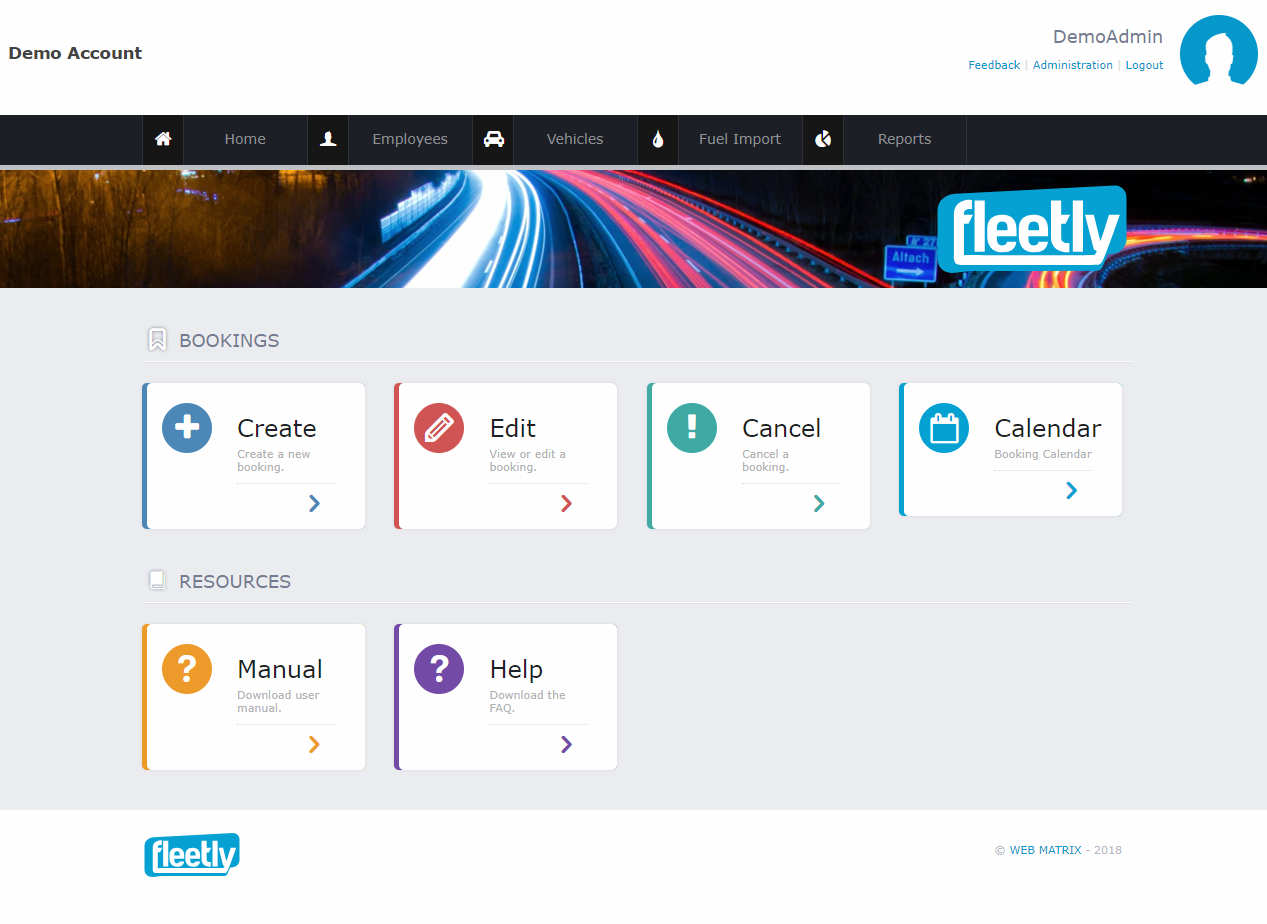
\includegraphics[width=\textwidth]{images/fleetly.png}
		\caption{Fleetly.}
	\end{figure}
	
	\section{Vinitysoft Fleet Manager}
	Kolejną popularną aplikacją jest \textit{Vinitysoft Fleet Manager} (\textit{https://www.vinitysoft.com/}). \textit{Vinitysoft Fleet Manager} kładzie mały nacisk na kontrolę dostępu do pojazdów i posiada system śledzenia towarów; jest to system przeznaczony dla firm których procesy główne opierają się na wykorzystywaniu samochodów. Interfejs użytkownika jest przestarzały i mało intuicyjny, ponadto często nie pozwala na wycofanie wprowadzonych zmian; wymaga czujności od użytkownika. Tak jak \textit{Fleetly}, \textit{Vinitysoft Fleet Manager} nie może zostać zintegrowany z zasobami firmy.
	\begin{figure}[H]
		\centering
		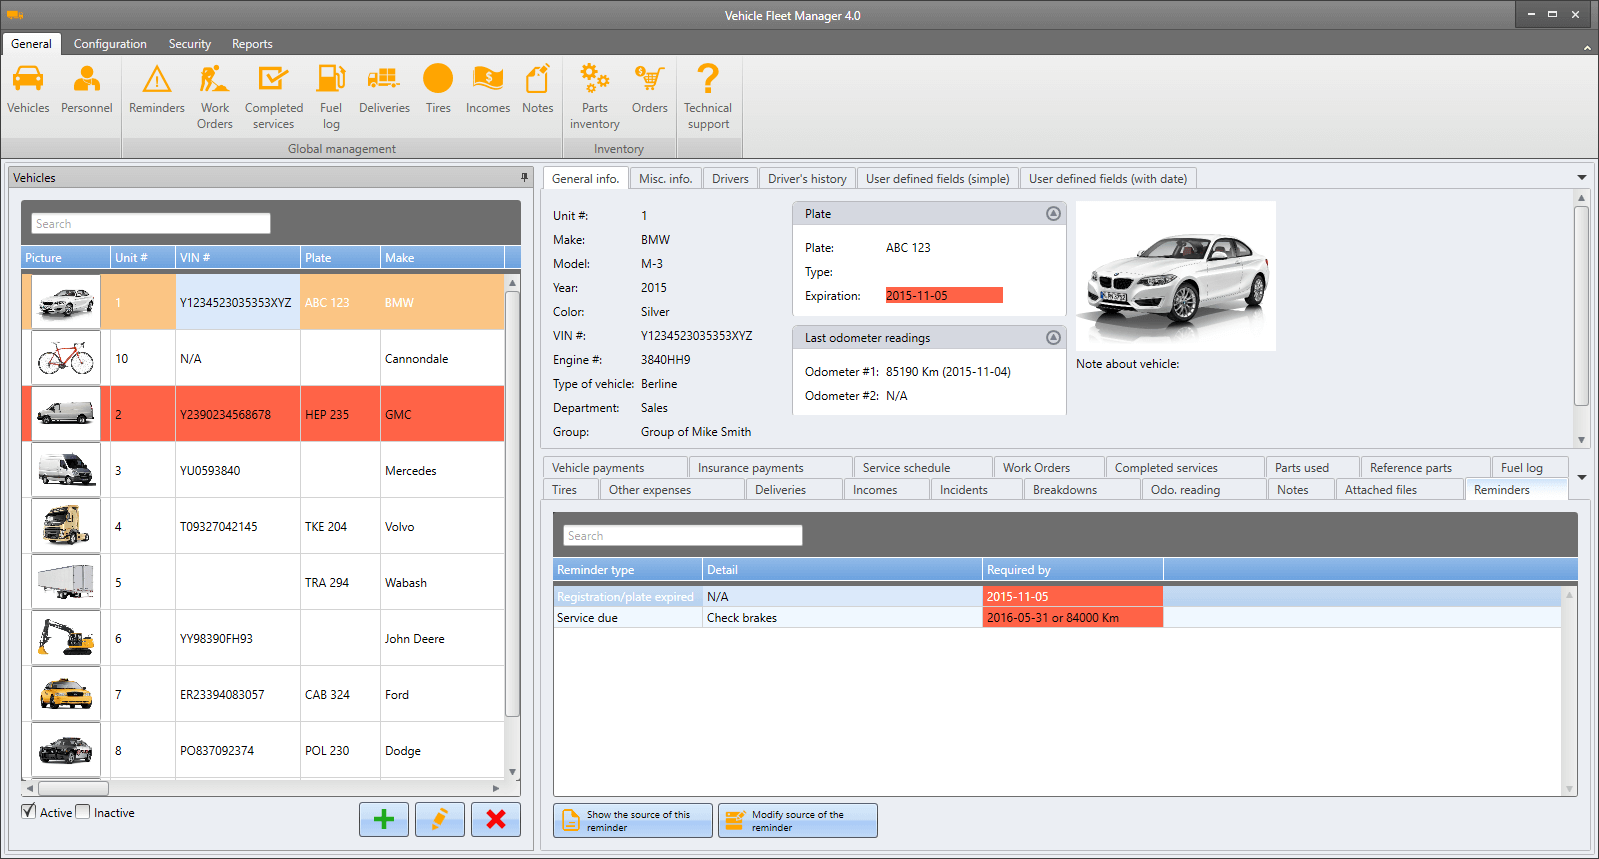
\includegraphics[width=\textwidth]{images/vinitysoft.png}
		\caption{Vinitysoft Fleet Management Software 4.0.}		
	\end{figure}
	%----------------------------------------------------------------------------------------
	%	SECTION 3
	%----------------------------------------------------------------------------------------
	\newpage
	\chapter{Wymagania funkcjonalne i niefunkcjonalne}
	\section{Wymagania funkcjonalne}
	System powinien pozwalać na:
	\begin{itemize}
		\item tworzenie nowych rezerwacji,
		\item kontrolę dostępu do pojazdów; utworzone rezerwację muszą być zaakceptowane przez kierowników,
		\item dodawanie, modyfikowanie oraz usuwanie informacji związanych z modelami pojazdów, pojazdami, ubezpieczeniami i naprawami,
		\item przechowywanie danych związanych z kosztami generowanymi przez flotę,
		\item monitorowanie akcji użytkowników (przechowywanie informacji o użytkownikach dokonujących modyfikacji danych).
	\end{itemize}
	Ponadto, system powinien korzystać z istniejących zasobów firmy (np. baz danych z danymi pracowników) by zredukować duplikację danych.
	
	
	
	\section{Wymagania niefunkcjonalne}
	\subsection{Interfejs użytkownika}
	Wymagania dotyczące wyglądu aplikacji są następujące:
	\begin{itemize}
		\item wygląd powinien być prosty i nowoczesny,
		\item elementy strony powinny być rozmieszczone w intuicyjny sposób,
		\item struktura widoków powinna być ułożona zgodnie z zależnościami między wyświetlanymi danymi,
		\item aplikacja powinna być wygodna w użyciu na ekranach komputerów o rozdzielczości HD (1366x768 pikseli) lub większej.
	\end{itemize}
	\newpage
	\subsection{Interfejs programistyczny}
	Wymagania dotyczące interfejsu programistycznego są następujące:
	\begin{itemize}
		\item system powinien wymagać niewielkich modyfikacji w przypadku integracji z istniejącymi zasobami firmy (np. baza danych pracowników),
		\item komunikacja powinna opierać się na otwartych i uniwersalnych standardach, np. dane w postaci \textit{JSON} lub \textit{XML} przesyłane protokołem \textit{HTTP},
		\item interfejs programistyczny powinien być niezależny od platformy tak by w przyszłości mógł zostać wykorzystany przez inne aplikacje.
	\end{itemize}
	\subsection{Bezpieczeństwo}
	System powinien być zabezpieczony zarówno po stronie interfejsu użytkownika (np. blokada przed przejściem do podstrony) oraz po stronie interfejsu programistycznego (ignorowanie zapytań od nieupoważnionych aplikacji). Zabezpieczenie powinno obsługiwać różne poziomy autoryzacji w zależności od roli użytkownika.
	
	%----------------------------------------------------------------------------------------
	%	SECTION 4
	%----------------------------------------------------------------------------------------
	\newpage
	\chapter{Zastosowane technologie i narzędzia}
	\section{Zastosowane technologie}
	Technologie wykorzystane w projekcie na chwilę obecną należą do czołówki platform dla aplikacji webowych.
	\subsection{Angular}
	Interfejs użytkownika wykorzystuje platformę \textit{Angular 7}. Podstawowymi elementami w \textit{Angular} są komponenty \cite{angular-components}, każdy z nich złożony z: pliku klasy \textit{TypeScript} zawierającej logikę, wzorca \textit{htm} opisującego wygląd widoku oraz opcjonalnego stylu \textit{css}; w przypadku jego braku styl brany jest z komponentu-rodzica. Warto zwrócić uwagę na język programowania wykorzystywany przez platformę \textit{Angular} — \textit{TypeScript} \cite{msdn-ts}, będący rozszerzeniem języka \textit{JavaScript}. \textit{TypeScript} dodaje silniejsze typowanie i kładzie większy nacisk na programowanie obiektowe, jednocześnie pozostając w pełni kompatybilnym z \textit{JavaScript}, do którego jest kompilowany. Proces kompilacji pozwala na usunięcie wielu błędów, które w przypadku \textit{JavaScript} zostałyby zauważone dopiero po uruchomieniu aplikacji.
	\begin{figure}[H]
		\centering
		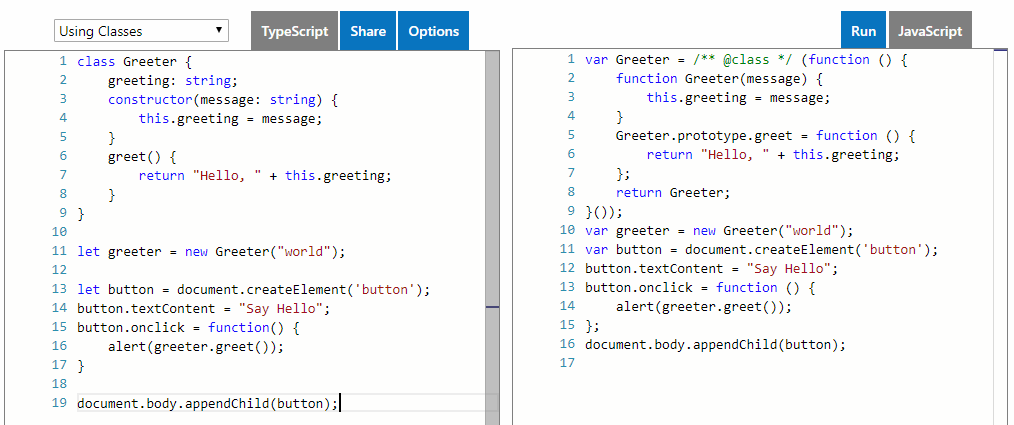
\includegraphics[width=\textwidth]{images/ts-to-js.png}
		\caption{Przykład kompilacji kodu TypeScript do JavaScript.}
		\small
		(\textit{http://www.typescriptlang.org})
	\end{figure}
	\subsection{Bootstrap}
	Jednym z ważniejszych komponentów aplikacji jest \textit{Bootstrap} - biblioteka interfejsu użytkownika pozwalająca w prosty sposób tworzyć estetyczne strony internetowe; poza wyglądem, \textit{Bootstrap} oferuje również wiele elementów \textit{UI} o zaawansowanej funkcjonalności w porównaniu do zwykłych odpowiedników.
	
	\subsection{ASP.NET Core i EF Core}
	Interfejs programistyczny oparty został na technologii \textit{ASP.NET Core 2.1} — jest to nowoczesna platforma oferująca działanie na wielu systemach operacyjnych oraz większa wydajność względem starszych rozwiązań firmy \textit{Microsoft}. Wykorzystany język programowania to obiektowy, kompilowany i statycznie typowany \textit{C\# 7.3}. Bardzo ważnym elementem tej części projektu jest \textit{EF (Entity Framework) Core 2.1} \cite{msdn-efcore}, framework \textit{ORM}  pozwalający na konwersję miedzy tabelami bazy danych a klasami \textit{C\#}. Jedną z najważniejszych funkcjonalności \textit{EF Core} jest wykorzystana w niniejszym projekcie możliwość utworzenia bazy danych przy użyciu konwencji \textit{Code First}; baza danych jest automatycznie generowana na podstawie klas \text{C\#} znajdujących się w projekcie. \textit{EF Core} współpracuje z większością popularnych baz danych; na potrzeby tego projektu wykorzystano \textit{MS SQL Server}.
	
	\section{Wykorzystane narzędzia}
	W trakcie realizacji projektu wykorzystane zostały narzędzia najczęściej używane przy wybranych technologiach.
	\subsection{Git}
	Do zarządzania kodem został wykorzystany system kontroli wersji \textit{Git}. Lokalna kopia projektu była synchronizowana ze zdalnym, prywatnym repozytorium znajdującym się na serwisie \text{GitHub}. Wykorzystane rozwiązanie pozwala na łatwy dostęp do wcześniejszych wersji projektu oraz zmniejsza ryzyko utraty kodu, gdyż nie jest on przechowywany tylko w jednym miejscu.
	\subsection{Visual Studio}
	Do rozwoju interfejsu programistycznego wykorzystano \textit{Visual Studio 2017}, flagowy produkt dla programistów od firmy \textit{Microsoft}. \textit{VS} pozwala na łatwe debugowanie kodu oraz analizę aspektów takich jak wykorzystanie zasobów przez program. Zaawansowany mechanizm podpowiedzi umożliwia sprawną pracę bez dokumentacji. \textit{Visual Studio} zostało wzbogacone o narzędzie \textit{JetBrains ReSharper} automatycznie formatujące pliki projektu według zadanego wzorca, zapewniając spójność i przejrzystość kodu. \textit{ReSharper} pozwala również na łatwiejsze uruchamianie i analizę testów.
	
	\subsection{Visual Studio Code}
	Aplikacja klienta była rozwijana przy użyciu \textit{Visual Studio Code 1.28}, nowoczesnego edytora firmy \textit{Microsoft}, który sprawdza się znakomicie przy tworzeniu interfejsów użytkownika ze względu na zintegrowaną konsolę pozwalającą na łatwe zarządzanie paczkami oraz łatwość dostosowywania do potrzeb użytkownika. W trakcie pracy wykorzystano wiele rozszerzeń, najważniejsze z nich to \textit{TSLint}, linter wykrywający błędy w kodzie \textit{TypeScript} oraz \textit{GitLens} — rozszerzenie wspomagające zarządzanie repozytorium \textit{Git}.
	

	\subsection{Postman}
	Interfejs programistyczny testowany był przy pomocy \textit{Postman 6.5.2}, aplikacji pozwalającej na wysyłanie oraz zarządzanie zapytaniami HTTP.
	
	%----------------------------------------------------------------------------------------
	%	SECTION 5
	%----------------------------------------------------------------------------------------
	\newpage
	\chapter{Projekt i implementacja}
	\section{Przypadki użycia}	
	Na podstawie wymagań funkcjonalnych opracowany został diagram przypadków użycia oraz szczegółowy opis wymaganej funkcjonalności.
	\begin{figure}[H]
		\centering
		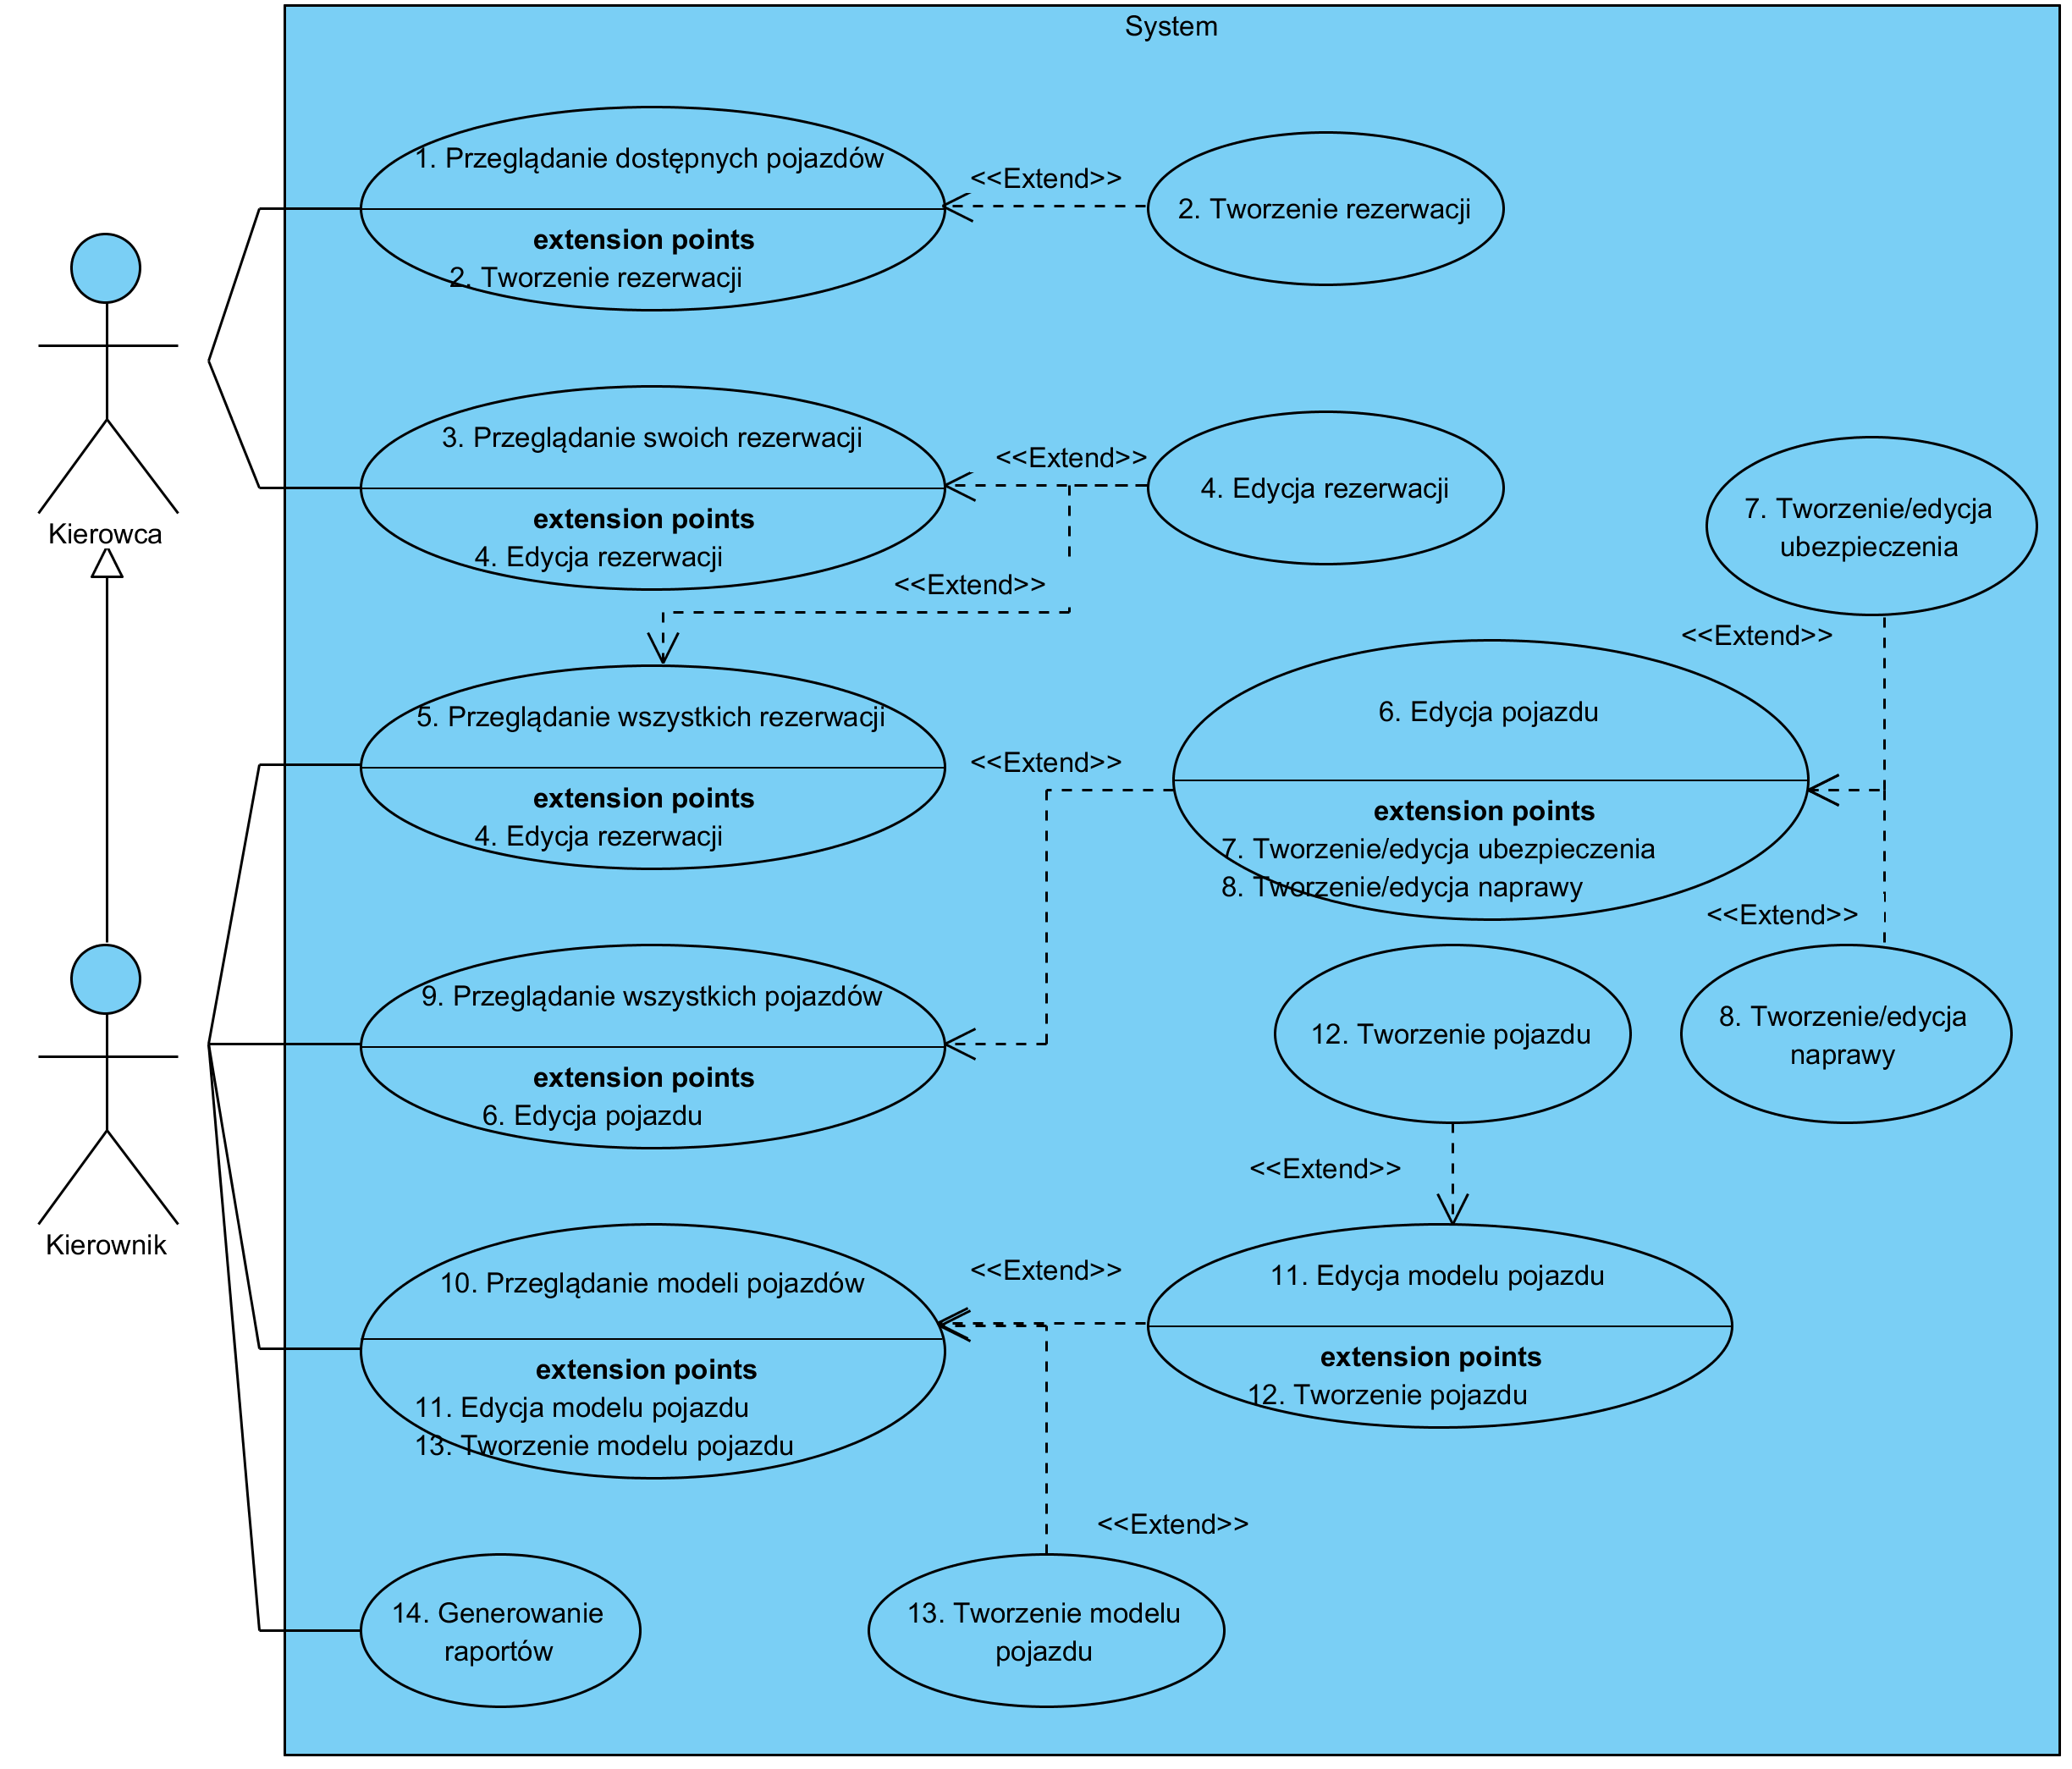
\includegraphics[width=\textwidth]{images/use_case_1.png}
		\caption{Diagram przypadków użycia.}
	\end{figure}
	\subsection{Szczegółowy opis przypadków użycia}
		Przypadki użycia zostały opisane według poniższego wzorca:
	\begin{table}[H]
		\begin{tabularx}{\textwidth}{|l|X|}
			\hline
			Numer                & Numer PU \\ \hline
			Nazwa                & Krótka nazwa (widoczna na diagramie)\\ \hline
			Opis                 & Dokładny opis\\ \hline
			Aktor                & Grupa użytkowników\\ \hline
			Kryterium spełnienia & Funkcjonalność, która musi zostać zaimplementowana by wymaganie można było uznać jako spełnione\\ \hline
			Ograniczenia         & Ograniczenia funkcjonalności, jeżeli takie istnieją\\ \hline
		\end{tabularx}
	\end{table}
	Rozróżniane są dwa rodzaje aktorów:
	\begin{itemize}
		\item Kierowca - użytkownik korzystający z funkcjonalności tworzenia i przeglądania historii rezerwacji.
		\item Kierownik - użytkownik z pełnym dostępem do systemu.
	\end{itemize}
	Kierownik posiada wszelkie prawa i możliwości Kierowcy.
	
	Dodatkowe pojęcia związane z modelami świata biznesowego:
	\begin{itemize}
		\item \textbf{Model Pojazdu} — model opisujący specyfikacje techniczną wspólną dla pewnego zbioru pojazdów.
		\item \textbf{Pojazd} — model opisujący informacje unikatowe dla pewnego przedstawiciela zbioru Modeli Pojazdów.
	\end{itemize}
	
	\begin{table}[H]
		\begin{tabularx}{\textwidth}{|l|X|}
			\hline
			Numer                & 1  \\ \hline
			Nazwa                & Przeglądanie dostępnych pojazdów \\ \hline
			Opis                 & System powinien pozwalać przeglądać listę dostępnych (możliwych do zarezerwowania) pojazdów. \\ \hline
			Aktor                & Kierowca \\ \hline
			Kryterium spełnienia & Kierowca może wyświetlić listę wszystkich dostępnych pojazdów oraz filtrować wyniki. \\ \hline
			Ograniczenia         &  \\ \hline
		\end{tabularx}
	\end{table}
	
	\begin{table}[H]
		\begin{tabularx}{\textwidth}{|l|X|}
			\hline
			Numer                & 2 \\ \hline
			Nazwa                & Tworzenie rezerwacji \\ \hline
			Opis                 & System powinien umożliwiać rezerwowanie dostępnych pojazdów, wyświetlonych w ramach \textbf{PU \#2}, wymagając wprowadzenia niezbędnych informacji jak okres i potrzeba stojąca za rezerwacją. \\ \hline
			Aktor                & Kierowca \\ \hline
			Kryterium spełnienia & Kierowca może utworzyć rezerwację. \\ \hline
			Ograniczenia         & Kierowca nie może utworzyć rezerwacji dla innego użytkownika. \\ \hline
		\end{tabularx}
	\end{table}	

	\begin{table}[H]
		\begin{tabularx}{\textwidth}{|l|X|}
			\hline
			Numer                & 3  \\ \hline
			Nazwa                & Przeglądanie swoich rezerwacji \\ \hline
			Opis                 & System powinien pozwalać przeglądać listę rezerwacji utworzonych przez obecnie zalogowanego użytkownika. \\ \hline
			Aktor                & Kierowca \\ \hline
			Kryterium spełnienia & Kierowca może wyświetlić listę rezerwacji które utworzył. \\ \hline
			Ograniczenia         &  \\ \hline
		\end{tabularx}
	\end{table}

	\begin{table}[H]
		\begin{tabularx}{\textwidth}{|l|X|}
			\hline
			Numer                & 4  \\ \hline
			Nazwa                & Edycja rezerwacji\\ \hline
			Opis                 & System powinien pozwalać edytować rezerwacje. Edycja pozwala na zmianę określonych pól w zależności od obecnego stanu i poziomu uprawnień zalogowanego użytkownika. \\ \hline
			Aktor                & Kierowca, Kierownik \\ \hline
			Kryterium spełnienia & Kierowca może wprowadzić podstawowe informacje dotyczące rezerwacji oraz przesłać ją do oceny kierownika. Po oddaniu samochodu kierowca może wpisać przejechane kilometry, zużyte paliwo oraz całkowitego koszt; po uzupełnieniu tych informacji rezerwacja może zostać oznaczona jako zakończona. Kierownik może zaakceptować lub odrzucić rezerwacje przesłane przez Kierowców. Kierownik ma również możliwość edycji większości pól, by mógł naprawić ew. błędy. \\ \hline
			Ograniczenia         & Jeżeli osobą tworzącą rezerwację jest użytkownik z uprawnieniami Kierownika, w ramach tego wypożyczenia może on podejmować wyłącznie działania wchodzące w rolę Kierowcy (np. nie może zaakceptować swojej rezerwacji). \\ \hline
		\end{tabularx}
	\end{table}

	\begin{table}[H]
		\begin{tabularx}{\textwidth}{|l|X|}
			\hline
			Numer                & 5  \\ \hline
			Nazwa                & Przeglądanie wszystkich rezerwacji \\ \hline
			Opis                 & System powinien pozwalać przeglądać listę wszystkich rezerwacji. \\ \hline
			Aktor                & Kierownik \\ \hline
			Kryterium spełnienia & Kierownik może wyświetlić listę wszystkich rezerwacji (niezależnie od stanu oraz użytkownika który rezerwację utworzyła) oraz filtrować wyniki. \\ \hline
			Ograniczenia         &  \\ \hline
		\end{tabularx}
	\end{table}	

	\begin{table}[H]
		\begin{tabularx}{\textwidth}{|l|X|}
			\hline
			Numer                & 6  \\ \hline
			Nazwa                & Przeglądanie wszystkich pojazdów \\ \hline
			Opis                 & System powinien pozwalać przeglądać listę pojazdów. \\ \hline
			Aktor                & Kierownik \\ \hline
			Kryterium spełnienia & Kierownik może wyświetlić listę pojazdów. \\ \hline
			Ograniczenia         &  \\ \hline
		\end{tabularx}
	\end{table}	

	\begin{table}[H]
		\begin{tabularx}{\textwidth}{|l|X|}
			\hline
			Numer                & 7  \\ \hline
			Nazwa                & Edycja pojazdów \\ \hline
			Opis                 & System powinien umożliwiać edycję pojazdów oraz wyświetlać powiązane informacje (ubezpieczenia i naprawy). \\ \hline
			Aktor                & Kierownik \\ \hline
			Kryterium spełnienia & Kierownik może wyświetlić szczegółowe informację na temat pojazdu oraz dokonać ich zmian. Kierownik może również przeglądać ubezpieczenia i naprawy powiązane z pojazdem. \\ \hline
			Ograniczenia         & Edycja pojazdu jest niemożliwa jeżeli pojazd jest zarezerwowany. Pojazd nie może zostać usunięty jeżeli był kiedykolwiek rezerwowany. \\ \hline
		\end{tabularx}
	\end{table}	

	\begin{table}[H]
		\begin{tabularx}{\textwidth}{|l|X|}
			\hline
			Numer                & 8  \\ \hline
			Nazwa                & Tworzenie/edycja ubezpieczenia \\ \hline
			Opis                 & System powinien umożliwiać tworzenie oraz późniejszą edycję ubezpieczeń. \\ \hline
			Aktor                & Kierownik \\ \hline
			Kryterium spełnienia & Kierownik może wprowadzić informacje związane z ubezpieczeniem pojazdu oraz edytować wcześniej utworzone ubezpieczenia. \\ \hline
			Ograniczenia         & Tworzenie/edycja ubezpieczeń nie jest możliwa dla pojazdu który jest zarezerwowany. \\ \hline
		\end{tabularx}
	\end{table}	

	\begin{table}[H]
		\begin{tabularx}{\textwidth}{|l|X|}
			\hline
			Numer                & 9  \\ \hline
			Nazwa                & Tworzenie/edycja naprawy \\ \hline
			Opis                 & System powinien umożliwiać tworzenie oraz późniejszą edycję napraw (zdarzeń serwisowych). \\ \hline
			Aktor                & Kierownik \\ \hline
			Kryterium spełnienia & Kierownik może wprowadzić informacje związane z naprawą pojazdu oraz edytować wcześniej utworzone naprawy. \\ \hline
			Ograniczenia         & Tworzenie/edycja napraw nie jest możliwa dla pojazdu który jest zarezerwowany. \\ \hline
		\end{tabularx}
	\end{table}	

	\begin{table}[H]
		\begin{tabularx}{\textwidth}{|l|X|}
			\hline
			Numer                & 10  \\ \hline
			Nazwa                & Przeglądanie modeli pojazdów \\ \hline
			Opis                 & System powinien pozwalać przeglądać listę modeli pojazdów. \\ \hline
			Aktor                & Kierownik \\ \hline
			Kryterium spełnienia & Kierownik może przeglądać modele pojazdów. \\ \hline
			Ograniczenia         & \\ \hline
		\end{tabularx}
	\end{table}	

	\begin{table}[H]
		\begin{tabularx}{\textwidth}{|l|X|}
			\hline
			Numer                & 11  \\ \hline
			Nazwa                & Edycja modelu pojazdu \\ \hline
			Opis                 & System powinien pozwalać przeglądać listę modeli pojazdów. \\ \hline
			Aktor                & Kierownik \\ \hline
			Kryterium spełnienia & Kierownik może dodawać modele pojazdów oraz edytować wcześniej utworzone modele. \\ \hline
			Ograniczenia         & Model pojazdu nie może zostać usunięty jeżeli system posiada egzemplarze danego modelu. \\ \hline
		\end{tabularx}
	\end{table}	

	\begin{table}[H]
		\begin{tabularx}{\textwidth}{|l|X|}
			\hline
			Numer                & 12  \\ \hline
			Nazwa                & Tworzenie pojazdu \\ \hline
			Opis                 & System powinien pozwalać na wprowadzanie informacji o pojazdach będących egzemplarzami wcześniej dodanych modeli. \\ \hline
			Aktor                & Kierownik \\ \hline
			Kryterium spełnienia & Kierownik może dodać nowy egzemplarz pojazdu  \\ \hline
			Ograniczenia         &  \\ \hline
		\end{tabularx}
	\end{table}	

	\begin{table}[H]
		\caption{Przypadek użycia: Generowanie raportów}
		\begin{tabularx}{\textwidth}{|l|X|}
			\hline
			Numer                & 13  \\ \hline
			Nazwa                & Tworzenie modelu pojazdu \\ \hline
			Opis                 & System powinien pozwalać na tworzenie modeli pojazdów. \\ \hline
			Aktor                & Kierownik \\ \hline
			Kryterium spełnienia & Kierownik może wprowadzać nowe modele pojazdów do systemu. \\ \hline
			Ograniczenia         &  \\ \hline
		\end{tabularx}
	\end{table}	

	\begin{table}[H]
		\caption{Przypadek użycia: Generowanie raportów}
		\begin{tabularx}{\textwidth}{|l|X|}
			\hline
			Numer                & 14  \\ \hline
			Nazwa                & Generowanie raportów \\ \hline
			Opis                 & System powinien umożliwiać eksportowanie kosztów generowanych przez flotę. Format raportu powinien być kompatybilny z programem \textit{Microsoft Excel}. \\ \hline
			Aktor                & Kierownik \\ \hline
			Kryterium spełnienia & System generuje raporty, z podziałem na rodzaj (raport dotyczący pojazdów, wypożyczeń itd.), Raporty mogą zostać zaimportowane do programu \textit{Microsoft Excel}; dane nie mogą wymagać skomplikowanych akcji ze strony użytkownika w celu utworzenia tabeli.\\ \hline
			Ograniczenia         &  \\ \hline
		\end{tabularx}
	\end{table}	

	\newpage
	\section{Architektura}
	System został stworzony przy użyciu klasycznej architektury, w której można wyodrębić trzy moduły - interfejs użytkownika (\textit{UI}), interfejs programistyczny (\textit{API}) oraz bazę danych (\textit{DB}). 
	
	\begin{figure}[H]
		\centering
		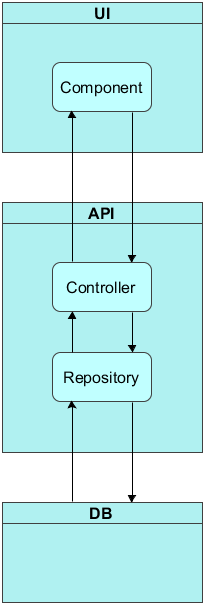
\includegraphics[scale=0.2]{images/architecture.png}
		\caption{Uproszczony schemat architektury z wyodrębnionymi najważniejszymi elementami składowymi.}
	\end{figure}	
	
	System został zaprojektowany tak, by mógł zostać zintegrowany z istniejącymi zasobami firmy — jedyne dane, jakie przechowuje, dotyczą logiki biznesowej, związanej z wymaganiami funkcjonalnymi; wynika to z faktu, że większość firm ma już własne bazy danych przechowujące informacje o pracownikach więc duplikacja danych jest niepożądana ze względu na zużycie zasobów oraz możliwe problemy z synchronizacją. Dane związane z użytkownikami (np. imię, nazwisko, e-mail i numer telefonu) czy lokacjami firmy (np. adres) mogą zostać pobrane z innej bazy danych; ponadto interfejs użytkownika nie umożliwia wprowadzania lub edycji takich danych. Implementacja opisana w dalszej części niniejszej pracy przechowuje przykładowe dane użytkowników do celów testowych w tej samej bazie danych, jednakże konfiguracja systemu tak by korzystał z innej, nie stanowi większego problemu.
	
	W architekturze można rozróżnić trzy najważniejsze składowe, dwie pierwsze w interfejsie programistycznym i trzecią w interfejsie użytkownika:
	\begin{itemize}
		\item Kontroler (\textit{Controller}) to klasa odpowiadająca za obsługę żądań \textit{HTTP} \cite{msdn-aspnet-api}.
		\item Repozytorium (\textit{Repository}) zawiera logikę pośredniczącą w komunikacji między \textit{API} a bazą danych.
		\item Komponent (\textit{Component}) to podstawowy element definiujący działanie widoku w \textit{Angular} \cite{angular-components}.
	\end{itemize}
	
	\section{Standardy}
	Projekt był tworzony zgodnie z dobrymi praktykami programowania, z naciskiem na poprawną implementację obiektowego paradygmatu programowania. Interfejs programistyczny był tworzony z użyciem sztandarowych możliwości języka C\# takimi jak typy ogólne \cite{msdn-generics} (\textit{Generics}) pozwalające na tworzenie pojedynczych metod i klas zdolnych do operacji na wielu typach, zachowując wszystkie zalety silnego, statycznego typowania i wysoką wydajność.
	
	W celu zapewnienia przejrzystości kodu, nazewnictwo wszystkich elementów oraz dokumentacja kodu są zgodne ze standardową konwencją danego języka. Kod jest napisany w całości w języku angielskim.
	\begin{table}[H]
		\caption{Najważniejsze konwencje nazewnicze.}
		\begin{tabularx}{\textwidth}{|l|l|l|l|X|}
			\hline
			Język      & Typy       			& Pliki                 & Zmienne prywatne & Inne zmienne \\ \hline
			C\# \cite{msdn-gnc}     & PascalCase & PascalCase.cs   		& camelCase        & PascalCase   \\ \hline
			TypeScript \cite{angular-sg} & PascalCase & snake-case.typ.ts 	& camelCase        & camelCase    \\ \hline
		\end{tabularx}
	\end{table}
	
	\newpage
	\section{Bezpieczeństwo}
	Dostęp do systemu został zabezpieczony przy użyciu standardu \textit{JWT} \cite{jwt}. Autoryzacja \textit{JWT} bazuje na generowaniu podpisanych (przez co odpornych na sfałszowanie) tokenów po stronie interfejsu programistycznego, a następnie wysyłaniu ich do aplikacji klienta. \textit{API} wymaga wcześniej wygenerowanego wymaga tokena w nagłówku \textit{HTTP} dla każdego żądania wysłanego przez interfejs użytkownika; żądania z niepoprawnym tokenem zostają odrzucone.
	
	Schemat działania autoryzacji \textit{JWT} w opisywanym projekcie wygląda następująco:
	\begin{enumerate}
		\item Użytkownik loguje się przez interfejs użytkownika, podając nazwę użytkownika oraz hasło
		\item Interfejs programistyczny weryfikuje dane logowania
		\item W przypadku prawidłowego hasła utworzony zostaje token \textit{JWT} zawierający:
		\subitem Informacje o wydającym token
		\subitem Informacje o użytkowniku: jego identyfikator (nazwa użytkownika) oraz role
		\item Utworzony token zostaje zaszyfrowany (uniemożliwiając jego sfałszowanie) i zwrócony	
		\item Odebrany token zostaje umieszczony w pamięci przeglądarki internetowej użytkownika
	\end{enumerate}
	Interfejs programistyczny weryfikuje poprawność tokena dla każdego żądania \textit{HTTP} z wyjątkiem tych związanych z procesem autoryzacji użytkownika; jeżeli token jest niepoprawny lub zbyt stary (wydany więcej niż 2 godziny przed weryfikacją), żądanie jest odrzucone; kod \textit{HTTP}: \textit{401 Unauthorized}.
	
	\begin{figure}[H]
		\centering
		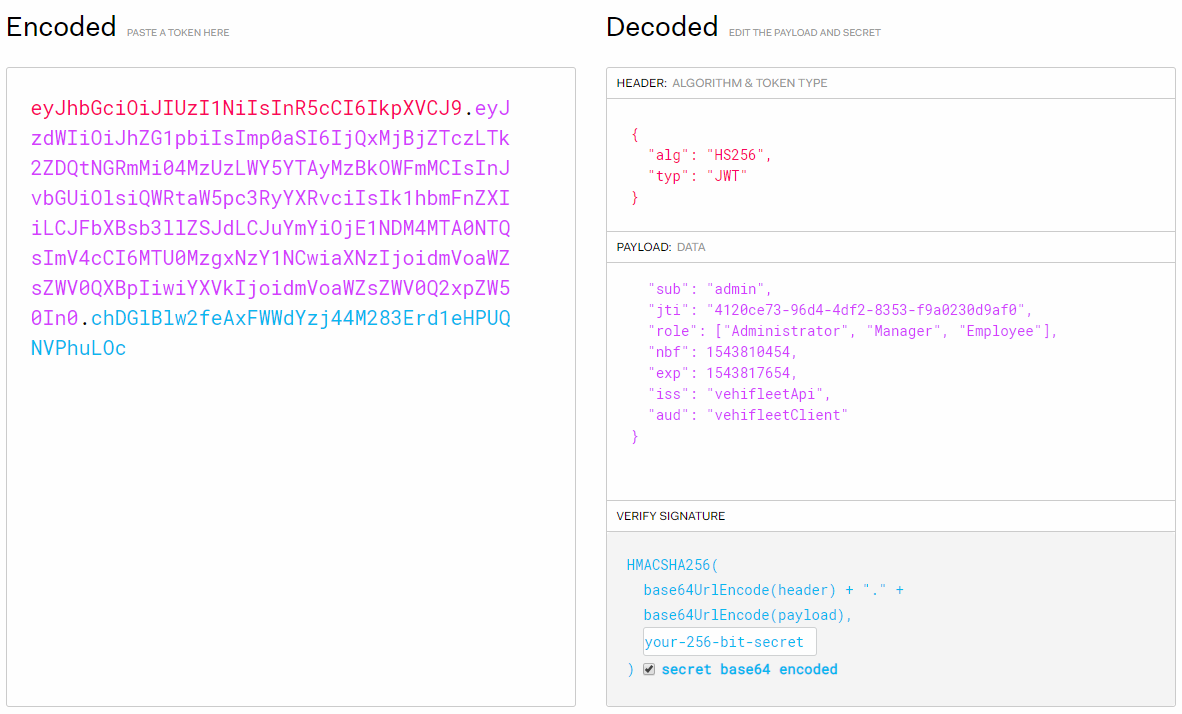
\includegraphics[width=\textwidth]{images/jwt.png}
		\caption{Przykładowy token \textit{JWT}.}
		\small 
		Token został wygenerowany przy użyciu narzędzia ze strony \textit{https://jwt.io/}.
	\end{figure}
	
	Przechowywanie ról w tokenie \textit{JWT} pozwala na autoryzację z uwzględnieniem uprawnień użytkownika, przykładowo, ograniczając dostęp do poufnych informacji lub modyfikacji przechowywanych danych przez osoby nieuprawnione.
	
	
	\begin{table}[H]
		\caption{Domyślna konfiguracja relacji ról do poziomu uprawnień.}
		\begin{tabularx}{\textwidth}{|l|l|X|}
			\hline
			\multicolumn{1}{|c|}{\textbf{Aktor}} & \multicolumn{1}{c|}{\textbf{Poziom dostępu}} & \multicolumn{1}{c|}{\textbf{Wymagane role}} \\ \hline
			Kierowca                             & Podstawowy                                   & Employee                                    \\ \hline
			Kierownik                            & Pełny                                        & Manager lub Administrator                   \\ \hline
		\end{tabularx}
	\end{table}
	
	Zarówno interfejs użytkownika jak i programistyczny utworzone w ramach projektu posiadają mechanizmy obrony przed nieautoryzowanym dostępem: \textit{API} zwraca błąd \textit{401 (Unauthorized)} dla żądań bez poprawnego tokena; Aplikacja użytkownika blokuje dostęp do widoków przy użyciu mechanizmu \textit{RouteGuard}.
	
	\newpage
	\section{Interfejs programistyczny}
	\subsection{Logika biznesowa}
	
	\begin{figure}[H]
		\centering
		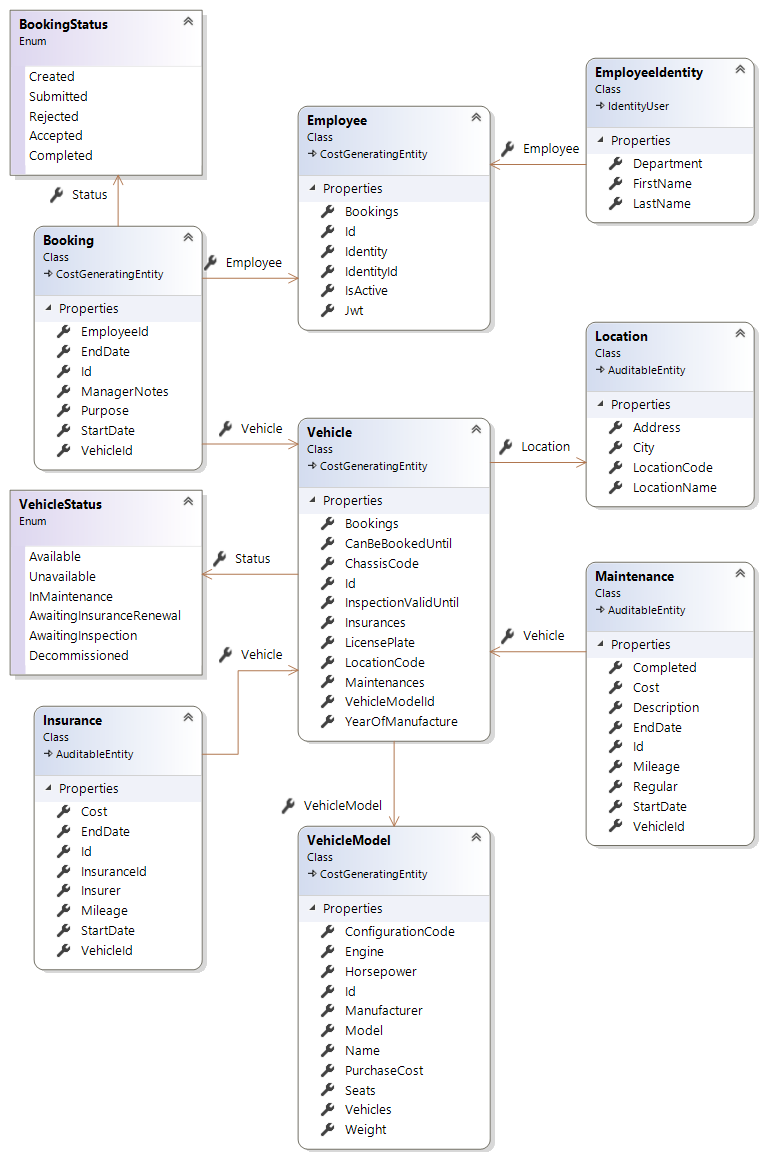
\includegraphics[width=\textwidth]{images/vs_class_diagram.png}
		\caption{Diagram klas.}
		\small 
		Diagram klas został wygenerowany przy użyciu \textit{Visual Studio}.
	\end{figure}
	
	\begin{table}[H]
		\caption{Klasy obiektów biznesowych.}
		\begin{tabularx}{\textwidth}{|l|X|}
			\hline
			\textbf{Klasa}   & \textbf{Opis}                                                                                              \\ \hline
			VehicleModel     & Specyfikacja techniczna wspólna dla wielu pojazdów                                                         \\ \hline
			Vehicle          & Informacje unikatowe dla pewnego pojazdu                                                                   \\ \hline
			Insurance        & Ubezpieczenie                                                                                              \\ \hline
			Maintenance      & Naprawa, serwis pojazdu                                                                                    \\ \hline
			Employee         & Klasa używana do powiązania logiki biznesowej z informacjami o pracowniku                                  \\ \hline
			EmployeeIdentity & Dane personalne użytkownika; mogą być pobierane z innej bazy danych                                        \\ \hline
			Booking          & Rezerwacja pojazdu                                                                                         \\ \hline
			Location         & Informacje o budynkach należących do firmy korzystającej z systemu; mogą być pobierane z innej bazy danych \\ \hline
		\end{tabularx}
	\end{table}

	Wszystkie klasy związane z logiką biznesową dziedziczą po klasie \textit{AuditableEntity} posiadającej pola przechowujące informacje (data i nazwa użytkownika) o utworzeniu i ostatniej edycji encji. Klasy związane z elementami generującymi koszty (pojazdami, modelami pojazdów, rezerwacjimi i użytkownikami) dziedziczą po klasie \textit{CostGeneratingEntity} przechowującej informacje o koszcie, zużytym paliwie i przejechanych kilometrach. 

	\lstinputlisting[language=C,frame=single,caption=Klasa abstrakcyjna AuditableEntity.]{source/efcore-auditable.cs}

	\lstinputlisting[language=C,frame=single,caption=Klasa abstrakcyjna CostGeneratingEntity.]{source/efcore-costgenerating.cs}
	
	\subsection{Baza danych}
	Baza danych została automatycznie wygenerowana na podstawie klas opisujących świat biznesowy, przy użyciu \textit{EF Core}. 
	
	Do zdefiniowania relacji między tabelami należało użyć pól typu takiego samego jak klucz główny docelowej klasy\cite{msdn-efcore-relationships}. Używanie adnotacji nie jest wymagane, o ile pole zostało nazwane według standardowej konwencji \textit{EF Core} — \textit{NazwaKlasyId} (np. \textit{VehicleId}). Dodatkowo klasę można uzupełnić o pola nawigacyjne (\textit{ang. navigation properties}), pozwalające na odnoszenie się do powiązanej klasy w łatwy sposób w kodzie programu, należy jednak pamiętać że domyślnie \textit{EF Core 2.1} nie wczytuje informacji o powiązanych obiektach; podczas komunikacji z bazą daną należy jawnie wywołać ładowanie powiązanych obiektów za pomocą metody \textit{LINQ} \text{Include()}.
	
%	Definiowanie właściwości kolumn wygenerowanych w bazie odbywa się poprzez umieszczenie odpowiednich adnotacji przy polach:
%	\begin{itemize}
%		\item $[$Key$]$: klucz główny (\textit{PK}),
%		\item $[$Required$]$: pole jest wymagane, nie może być puste (null).
%	\end{itemize}
	
	\lstinputlisting[language=C,frame=single,caption=Przykład definiowania relacji między klasami w code-first.]{source/efcore-model.cs}
	
	\lstinputlisting[language=C,frame=single,caption=Ładowanie powiązanych obiektów na przykładzie relacji rezerwacji do pojazdu.]{source/efcore-loading-related.cs}
	
	Wybrana strategia dziedziczenia to \textit{TPC — Table per Concrete Type}. W strategii \textit{TPC} tabele utworzone w bazie danych zawierają wszystkie kolumny odpowiadające polom wszystkich klas w hierarchii dziedziczenia.
	
	\newpage
	\subsection{Struktura solucji}
	Kod interfejsu programistycznego znajduje się w jednej solucji podzielonej na projekty.
	\begin{itemize}
		\item \textbf{Vehifleet} — solucja
		\subitem \textbf{Vehifleet.API} — konfiguracja systemu oraz kontrolery; projekt startowy
		\subitem \textbf{Vehifleet.API.QueryFilters} — filtry używane w żądaniach GET
		\subitem \textbf{Vehifleet.Data.DbAccess} — konfiguracja połączenia z bazą danych
		\subitem \textbf{Vehifleet.Data.Dtos} — modele transportowe (\textit{ang. Data Transfer Objects}) używane w komunikacji z interfejsem użytkownika
		\subitem \textbf{Vehifleet.Data.Models} — modele używane wewnątrz interfejsu programistycznego oraz przy tworzeniu bazy danych
		\subitem \textbf{Vehifleet.Helper} — pomocnicze metody rozszerzające \cite{msdn-extension}
		\subitem \textbf{Vehifleet.Repositories} — repozytoria odpowiedzialne za interakcje z bazą danych
		\subitem \textbf{Vehifleet.Services.UserService} — obsługa logowania użytkowników
		\subitem \textbf{Vehifleet.Services.CsvService} — serwis generujący raporty ze statystkami
	\end{itemize}

	\subsection{Wstrzykiwanie zależności}
	Obiekty klas z logiką są tworzone przy użyciu wstrzykiwania zależności (\textit{ang. dependency injection}). Większość obiektów jest tworzona dla konkretnego żądania odebranego przez kontroler; po wykonaniu operacji i zwróceniu odpowiedzi obiekt trafia do puli oczekującej na \textit{GC}.
	
	\subsection{Kontrolery}
	Jednymi z najważniejszych klas są kontrolery, komponenty obsługujące żądania \textit{HTTP}. Logika z różnych projektów jest łączona i używana w klasach kontrolerów. 
	Poniżej zamieszczony został opis wszystkich punktów końcowych (\textit{ang. endpoint}) w interfejsie programistycznym.
	%----------------------------------------------------------------------------------------
	\begin{table}[H]
	\caption{Endpoint \textit{api/vehicle-models GET}.}
	\begin{tabularx}{\textwidth}{|l|l|X|}
		\hline
		\multicolumn{3}{|c|}{\textbf{\textbf{Opis}}}
		\\ \hline
		\textbf{URL}                         & \multicolumn{2}{l|}{api/vehicle-models}
		\\ \hline
		\textbf{Wymagane role}               & \multicolumn{2}{l|}{Employee}
		\\ \hline
		\textbf{Metoda}                      & \multicolumn{2}{l|}{GET}
		\\ \hline
		\multicolumn{3}{|c|}{ Odpowiedzi}
		\\ \hline
		\multirow{2}{*}{200 (OK)}   & \textbf{Zawartość}         & Tablica \textit{JSON}
		\\ \cline{2-3}              & \textbf{Opis}         	    & Lista modeli pojazdów
		\\ \hline
	\end{tabularx}
\end{table}

\begin{table}[H]
	\caption{Endpoint \textit{api/vehicle-models/manufacturers GET}.}
	\begin{tabularx}{\textwidth}{|l|l|X|}
		\hline
		\multicolumn{3}{|c|}{\textbf{\textbf{Opis}}}
		
		\\ \hline
		\textbf{URL}                         & \multicolumn{2}{l|}{api/vehicle-models/manufacturers}
		\\ \hline
		\textbf{Wymagane role}               & \multicolumn{2}{l|}{Employee}
		\\ \hline
		\textbf{Metoda}                      & \multicolumn{2}{l|}{GET}
		\\ \hline
		\multicolumn{3}{|c|}{\textbf{Odpowiedzi}}
		\\ \hline
		\multirow{2}{*}{200 (OK)}   & \textbf{Zawartość}        & Tablica \textit{JSON}
		\\ \cline{2-3}              & \textbf{Opis}         	   & Lista marek pojazdów
		\\ \hline
	\end{tabularx}
\end{table}

\begin{table}[H]
	\caption{Endpoint \textit{api/vehicle-models/id GET}.}
	\begin{tabularx}{\textwidth}{|l|l|X|}
		\hline
		\multicolumn{3}{|c|}{\textbf{\textbf{Opis}}}
		\\ \hline
		\textbf{URL}                         & \multicolumn{2}{l|}{api/vehicle-models/id}
		\\ \hline
		\textbf{Wymagane role}               & \multicolumn{2}{l|}{Employee}
		\\ \hline
		\textbf{Metoda}                      & \multicolumn{2}{l|}{GET}
		\\ \hline
		\multicolumn{3}{|c|}{\textbf{Odpowiedzi}}
		\\ \hline
		\multirow{2}{*}{200 (OK)} 	        & \textbf{Zawartość}   	& \textit{JSON}
		\\ \cline{2-3}                      & \textbf{Opis}         	& Model pojazdu o żądanym \textit{id}
		\\ \hline
		\multirow{2}{*}{404 (Not Found)} 	& \textbf{Zawartość}     & \lstinputlisting[language=json,nolol=true]{source/vehicle-models-get-by-id-404.json}
		\\ \cline{2-3}                      & \textbf{Opis}          & Model pojazdu o żądanym \textit{id} nie istnieje
		\\ \hline
	\end{tabularx}
\end{table}

\begin{table}[H]
	\caption{Endpoint \textit{api/vehicle-models POST}.}
	\begin{tabularx}{\textwidth}{|l|l|X|}
		\hline
		\multicolumn{3}{|c|}{\textbf{\textbf{Opis}}}
		\\ \hline
		\textbf{URL}                       & \multicolumn{2}{l|}{api/vehicle-models}
		\\ \hline
		\textbf{Wymagane role}             & \multicolumn{2}{l|}{Employee}
		\\ \hline
		\textbf{Metoda}                    & \multicolumn{2}{l|}{POST}
		\\ \hline
		\multicolumn{3}{|c|}{\textbf{Odpowiedzi}}
		\\ \hline
		\multirow{2}{*}{200 (OK)} 		& \textbf{Zawartość}     & \textit{Id} utworzonego modelu pojazdu
		\\ \cline{2-3}                  & \textbf{Opis}         	& Model pojazdu został utworzony
		\\ \hline
	\end{tabularx}
\end{table}

\begin{table}[H]
	\caption{Endpoint \textit{api/vehicle-models/id PUT}.}
	\begin{tabularx}{\textwidth}{|l|l|X|}
		\hline
		\multicolumn{3}{|c|}{\textbf{\textbf{Opis}}}
		\\ \hline
		\textbf{URL}                       & \multicolumn{2}{l|}{api/vehicle-models/id}
		\\ \hline
		\textbf{Wymagane role}             & \multicolumn{2}{l|}{Manager, Administrator}
		\\ \hline
		\textbf{Metoda}                    & \multicolumn{2}{l|}{PUT}
		\\ \hline
		\multicolumn{3}{|c|}{\textbf{Odpowiedzi}}
		\\ \hline
		200 (OK) 		 & \textbf{Opis}      	& Model pojazdu został zaktualizowany
		\\ \hline
		\multirow{2}{*}{404 (Not Found)} 	    & \textbf{Zawartość}     & \lstinputlisting[language=json,nolol=true]{source/vehicle-models-put-404.json}  
		\\ \cline{2-3}                          & \textbf{Opis}          & Model pojazdu o żądanym \textit{id} nie istnieje
		\\ \hline
	\end{tabularx}
\end{table}

\begin{table}[H]
	\caption{Endpoint \textit{api/vehicle-models/id DELETE}.}
	\begin{tabularx}{\textwidth}{|l|l|X|}
		\hline
		\multicolumn{3}{|c|}{\textbf{\textbf{Opis}}}
		\\ \hline
		\textbf{URL}                       & \multicolumn{2}{l|}{api/vehicle-models/id}
		\\ \hline
		\textbf{Wymagane role}             & \multicolumn{2}{l|}{Manager, Administrator}
		\\ \hline
		\textbf{Metoda}                    & \multicolumn{2}{l|}{DELETE}
		\\ \hline
		\multicolumn{3}{|c|}{\textbf{Odpowiedzi}}
		\\ \hline
		200 (OK)			                & \textbf{Opis}         	& Model pojazdu został usunięty
		\\ \hline
		\multirow{2}{*}{404 (Not Found)} 	& \textbf{Zawartość}     & \lstinputlisting[language=json,nolol=true]{source/vehicle-models-delete-404.json}   	
		\\ \cline{2-3}                      & \textbf{Opis}          & Model pojazdu o żądanym \textit{id} nie istnieje
		\\ \hline
		\multirow{2}{*}{400 (Bad Request)} 	& \textbf{Zawartość}     & \lstinputlisting[language=json,nolol=true]{source/vehicle-models-delete-400.json}   	
		\\ \cline{2-3}                      & \textbf{Opis}          & System posiada egzemplarze modelu pojazdu o żądanym \textit{id}, nie może on zostać usunięty
		\\ \hline
	\end{tabularx}
\end{table}

%----------------------------------------------------------------------------------------
\begin{table}[H]
	\caption{Endpoint \textit{api/vehicles GET}.}
	\begin{tabularx}{\textwidth}{|l|l|X|}
		\hline
		\multicolumn{3}{|c|}{\textbf{\textbf{Opis}}}
		\\ \hline
		\textbf{URL}                         & \multicolumn{2}{l|}{api/vehicles}
		\\ \hline
		\textbf{Wymagane role}               & \multicolumn{2}{l|}{Employee}
		\\ \hline
		\textbf{Metoda}                      & \multicolumn{2}{l|}{GET}
		\\ \hline
		\multicolumn{3}{|c|}{ Odpowiedzi}
		\\ \hline
		\multirow{2}{*}{200 (OK)}   & \textbf{Zawartość}         & Tablica \textit{JSON}
		\\ \cline{2-3}              & \textbf{Opis}         	    & Lista pojazdów
		\\ \hline
	\end{tabularx}
\end{table}

\begin{table}[H]
	\caption{Endpoint \textit{api/vehicles/id GET}.}
	\begin{tabularx}{\textwidth}{|l|l|X|}
		\hline
		\multicolumn{3}{|c|}{\textbf{\textbf{Opis}}}
		\\ \hline
		\textbf{URL}                         & \multicolumn{2}{l|}{api/vehicles/id}
		\\ \hline
		\textbf{Wymagane role}               & \multicolumn{2}{l|}{Employee}
		\\ \hline
		\textbf{Metoda}                      & \multicolumn{2}{l|}{GET}
		\\ \hline
		\multicolumn{3}{|c|}{\textbf{Odpowiedzi}}
		\\ \hline
		\multirow{2}{*}{200 (OK)} 	        & \textbf{Zawartość}   	& \textit{JSON}
		\\ \cline{2-3}                      & \textbf{Opis}         	& Pojazd o żądanym \textit{id}
		\\ \hline
		\multirow{2}{*}{404 (Not Found)} 	& \textbf{Zawartość}     & \lstinputlisting[language=json,nolol=true]{source/vehicles-get-by-id-404.json}
		\\ \cline{2-3}                      & \textbf{Opis}          & Pojazd o żądanym \textit{id} nie istnieje
		\\ \hline
	\end{tabularx}
\end{table}

\begin{table}[H]
	\caption{Endpoint \textit{api/vehicles POST}.}
	\begin{tabularx}{\textwidth}{|l|l|X|}
		\hline
		\multicolumn{3}{|c|}{\textbf{\textbf{Opis}}}
		\\ \hline
		\textbf{URL}                       & \multicolumn{2}{l|}{api/vehicles}
		\\ \hline
		\textbf{Wymagane role}             & \multicolumn{2}{l|}{Manager, Administrator}
		\\ \hline
		\textbf{Metoda}                    & \multicolumn{2}{l|}{POST}
		\\ \hline
		\multicolumn{3}{|c|}{\textbf{Odpowiedzi}}
		\\ \hline
		\multirow{2}{*}{200 (OK)} 		& \textbf{Zawartość}     & \textit{Id} utworzonego pojazdu
		\\ \cline{2-3}                  & \textbf{Opis}         	& Pojazd został utworzony
		\\ \hline
	\end{tabularx}
\end{table}

\begin{table}[H]
	\caption{Endpoint \textit{api/vehicles/id PUT}.}
	\begin{tabularx}{\textwidth}{|l|l|X|}
		\hline
		\multicolumn{3}{|c|}{\textbf{\textbf{Opis}}}
		\\ \hline
		\textbf{URL}                       & \multicolumn{2}{l|}{api/vehicles/id}
		\\ \hline
		\textbf{Wymagane role}             & \multicolumn{2}{l|}{Manager, Administrator}
		\\ \hline
		\textbf{Metoda}                    & \multicolumn{2}{l|}{PUT}
		\\ \hline
		\multicolumn{3}{|c|}{\textbf{Odpowiedzi}}
		\\ \hline
		200 (OK) 		                        & \textbf{Opis}      	& Pojazd zostało zaktualizowane
		\\ \hline
		\multirow{2}{*}{404 (Not Found)} 	    & \textbf{Zawartość}     & \lstinputlisting[language=json,nolol=true]{source/vehicles-put-404.json}  
		\\ \cline{2-3}                          & \textbf{Opis}          & Pojazd o żądanym \textit{id} nie istnieje
		\\ \hline
	\end{tabularx}
\end{table}

\begin{table}[H]
	\caption{Endpoint \textit{api/vehicles/id DELETE}.}
	\begin{tabularx}{\textwidth}{|l|l|X|}
		\hline
		\multicolumn{3}{|c|}{\textbf{\textbf{Opis}}}
		\\ \hline
		\textbf{URL}                       & \multicolumn{2}{l|}{api/vehicles/id}
		\\ \hline
		\textbf{Wymagane role}             & \multicolumn{2}{l|}{Manager, Administrator}
		\\ \hline
		\textbf{Metoda}                    & \multicolumn{2}{l|}{DELETE}
		\\ \hline
		\multicolumn{3}{|c|}{\textbf{Odpowiedzi}}
		\\ \hline
		200 (OK)			                & \textbf{Opis}         	& Pojazd został usunięty
		\\ \hline
		\multirow{2}{*}{404 (Not Found)} 	& \textbf{Zawartość}     & \lstinputlisting[language=json,nolol=true]{source/vehicles-delete-404.json}   	
		\\ \cline{2-3}                      & \textbf{Opis}          & Pojazd o żądanym \textit{id} nie istnieje
		\\ \hline
		\multirow{2}{*}{400 (Bad Request)} 	& \textbf{Zawartość}     & \lstinputlisting[language=json,nolol=true]{source/vehicles-delete-400.json}   	
		\\ \cline{2-3}                      & \textbf{Opis}          & System posiada rezerwacje przypisane do pojazdu o żądanym \textit{id}, nie może on zostać usunięty
		\\ \hline
	\end{tabularx}
\end{table}

%----------------------------------------------------------------------------------------
\begin{table}[H]
	\caption{Endpoint \textit{api/insurances/vehicle/id GET}.}
	\begin{tabularx}{\textwidth}{|l|l|X|}
		\hline
		\multicolumn{3}{|c|}{\textbf{\textbf{Opis}}}
		\\ \hline
		\textbf{URL}                         & \multicolumn{2}{l|}{api/insurances/vehicle/id}
		\\ \hline
		\textbf{Wymagane role}               & \multicolumn{2}{l|}{Employee}
		\\ \hline
		\textbf{Metoda}                      & \multicolumn{2}{l|}{GET}
		\\ \hline
		\multicolumn{3}{|c|}{ Odpowiedzi}
		\\ \hline
		\multirow{2}{*}{200 (OK)}   & \textbf{Zawartość}         & Tablica \textit{JSON}
		\\ \cline{2-3}              & \textbf{Opis}         	    & Lista ubezpieczeń przypisanych do danego pojazdu
		\\ \hline
	\end{tabularx}
\end{table}

\begin{table}[H]
	\caption{Endpoint \textit{api/insurances/id GET}.}
	\begin{tabularx}{\textwidth}{|l|l|X|}
		\hline
		\multicolumn{3}{|c|}{\textbf{\textbf{Opis}}}
		\\ \hline
		\textbf{URL}                         & \multicolumn{2}{l|}{api/insurances/id}
		\\ \hline
		\textbf{Wymagane role}               & \multicolumn{2}{l|}{Employee}
		\\ \hline
		\textbf{Metoda}                      & \multicolumn{2}{l|}{GET}
		\\ \hline
		\multicolumn{3}{|c|}{\textbf{Odpowiedzi}}
		\\ \hline
		\multirow{2}{*}{200 (OK)} 	        & \textbf{Zawartość}   	& \textit{JSON}
		\\ \cline{2-3}                      & \textbf{Opis}         	& Ubezpieczenie o żądanym \textit{id}
		\\ \hline
		\multirow{2}{*}{404 (Not Found)} 	& \textbf{Zawartość}     & \lstinputlisting[language=json,nolol=true]{source/insurances-get-by-id-404.json}
		\\ \cline{2-3}                      & \textbf{Opis}          & Ubezpieczenie o żądanym \textit{id} nie istnieje
		\\ \hline
	\end{tabularx}
\end{table}

\begin{table}[H]
	\caption{Endpoint \textit{api/insurances POST}.}
	\begin{tabularx}{\textwidth}{|l|l|X|}
		\hline
		\multicolumn{3}{|c|}{\textbf{\textbf{Opis}}}
		\\ \hline
		\textbf{URL}                       & \multicolumn{2}{l|}{api/insurances}
		\\ \hline
		\textbf{Wymagane role}             & \multicolumn{2}{l|}{Manager, Administrator}
		\\ \hline
		\textbf{Metoda}                    & \multicolumn{2}{l|}{POST}
		\\ \hline
		\multicolumn{3}{|c|}{\textbf{Odpowiedzi}}
		\\ \hline
		\multirow{2}{*}{200 (OK)} 		& \textbf{Zawartość}     & \textit{Id} utworzonego ubezpieczenia
		\\ \cline{2-3}                  & \textbf{Opis}         	& Ubezpieczenie został utworzony
		\\ \hline
	\end{tabularx}
\end{table}

\begin{table}[H]
	\caption{Endpoint \textit{api/insurances/id PUT}.}
	\begin{tabularx}{\textwidth}{|l|l|X|}
		\hline
		\multicolumn{3}{|c|}{\textbf{\textbf{Opis}}}
		\\ \hline
		\textbf{URL}                       & \multicolumn{2}{l|}{api/insurances/id}
		\\ \hline
		\textbf{Wymagane role}             & \multicolumn{2}{l|}{Manager, Administrator}
		\\ \hline
		\textbf{Metoda}                    & \multicolumn{2}{l|}{PUT}
		\\ \hline
		\multicolumn{3}{|c|}{\textbf{Odpowiedzi}}
		\\ \hline
		200 (OK) 		                        & \textbf{Opis}      	& Ubezpieczenie zostało zaktualizowane
		\\ \hline
		\multirow{2}{*}{404 (Not Found)} 	    & \textbf{Zawartość}     & \lstinputlisting[language=json,nolol=true]{source/insurances-put-404.json}
		\\ \cline{2-3}                          & \textbf{Opis}          & Ubezpieczenie o żądanym \textit{id} nie istnieje
		\\ \hline
	\end{tabularx}
\end{table}

\begin{table}[H]
	\caption{Endpoint \textit{api/insurances/id DELETE}.}
	\begin{tabularx}{\textwidth}{|l|l|X|}
		\hline
		\multicolumn{3}{|c|}{\textbf{\textbf{Opis}}}
		\\ \hline
		\textbf{URL}                       & \multicolumn{2}{l|}{api/insurances/id}
		\\ \hline
		\textbf{Wymagane role}             & \multicolumn{2}{l|}{Manager, Administrator}
		\\ \hline
		\textbf{Metoda}                    & \multicolumn{2}{l|}{DELETE}
		\\ \hline
		\multicolumn{3}{|c|}{\textbf{Odpowiedzi}}
		\\ \hline
		200 (OK)			                & \textbf{Opis}         	& Ubezpieczenie został usunięty
		\\ \hline
		\multirow{2}{*}{404 (Not Found)} 	& \textbf{Zawartość}     & \lstinputlisting[language=json,nolol=true]{source/insurances-delete-404.json}
		\\ \cline{2-3}                      & \textbf{Opis}          & Ubezpieczenie o żądanym \textit{id} nie istnieje
		\\ \hline
	\end{tabularx}
\end{table}

%----------------------------------------------------------------------------------------
\begin{table}[H]
	\caption{Endpoint \textit{api/maintenances/vehicle/id GET}.}
	\begin{tabularx}{\textwidth}{|l|l|X|}
		\hline
		\multicolumn{3}{|c|}{\textbf{\textbf{Opis}}}
		\\ \hline
		\textbf{URL}                         & \multicolumn{2}{l|}{api/maintenances/vehicle/id}
		\\ \hline
		\textbf{Wymagane role}               & \multicolumn{2}{l|}{Employee}
		\\ \hline
		\textbf{Metoda}                      & \multicolumn{2}{l|}{GET}
		\\ \hline
		\multicolumn{3}{|c|}{ Odpowiedzi}
		\\ \hline
		\multirow{2}{*}{200 (OK)}   & \textbf{Zawartość}         & Tablica \textit{JSON}
		\\ \cline{2-3}              & \textbf{Opis}         	    & Lista napraw przypisanych do danego pojazdu
		\\ \hline
	\end{tabularx}
\end{table}

\begin{table}[H]
	\caption{Endpoint \textit{api/maintenances/id GET}.}
	\begin{tabularx}{\textwidth}{|l|l|X|}
		\hline
		\multicolumn{3}{|c|}{\textbf{\textbf{Opis}}}
		\\ \hline
		\textbf{URL}                         & \multicolumn{2}{l|}{api/maintenances/id}
		\\ \hline
		\textbf{Wymagane role}               & \multicolumn{2}{l|}{Employee}
		\\ \hline
		\textbf{Metoda}                      & \multicolumn{2}{l|}{GET}
		\\ \hline
		\multicolumn{3}{|c|}{\textbf{Odpowiedzi}}
		\\ \hline
		\multirow{2}{*}{200 (OK)} 	        & \textbf{Zawartość}   	& \textit{JSON}
		\\ \cline{2-3}                      & \textbf{Opis}         	& Naprawa o żądanym \textit{id}
		\\ \hline
		\multirow{2}{*}{404 (Not Found)} 	& \textbf{Zawartość}     & \lstinputlisting[language=json,nolol=true]{source/maintenances-get-by-id-404.json}
		\\ \cline{2-3}                      & \textbf{Opis}          & Naprawa o żądanym \textit{id} nie istnieje
		\\ \hline
	\end{tabularx}
\end{table}

\begin{table}[H]
	\caption{Endpoint \textit{api/maintenances POST}.}
	\begin{tabularx}{\textwidth}{|l|l|X|}
		\hline
		\multicolumn{3}{|c|}{\textbf{\textbf{Opis}}}
		\\ \hline
		\textbf{URL}                       & \multicolumn{2}{l|}{api/maintenances}
		\\ \hline
		\textbf{Wymagane role}             & \multicolumn{2}{l|}{Manager, Administrator}
		\\ \hline
		\textbf{Metoda}                    & \multicolumn{2}{l|}{POST}
		\\ \hline
		\multicolumn{3}{|c|}{\textbf{Odpowiedzi}}
		\\ \hline
		\multirow{2}{*}{200 (OK)} 		& \textbf{Zawartość}     & \textit{Id} utworzonego ubezpieczenia
		\\ \cline{2-3}                  & \textbf{Opis}         	& Naprawa została utworzona
		\\ \hline
	\end{tabularx}
\end{table}

\begin{table}[H]
	\caption{Endpoint \textit{api/maintenances/id PUT}.}
	\begin{tabularx}{\textwidth}{|l|l|X|}
		\hline
		\multicolumn{3}{|c|}{\textbf{\textbf{Opis}}}
		\\ \hline
		\textbf{URL}                       & \multicolumn{2}{l|}{api/maintenances/id}
		\\ \hline
		\textbf{Wymagane role}             & \multicolumn{2}{l|}{Manager, Administrator}
		\\ \hline
		\textbf{Metoda}                    & \multicolumn{2}{l|}{PUT}
		\\ \hline
		\multicolumn{3}{|c|}{\textbf{Odpowiedzi}}
		\\ \hline
		200 (OK) 		                        & \textbf{Opis}      	& Naprawa została zauktualizowana
		\\ \hline
		\multirow{2}{*}{404 (Not Found)} 	    & \textbf{Zawartość}     & \lstinputlisting[language=json,nolol=true]{source/maintenances-put-404.json}
		\\ \cline{2-3}                          & \textbf{Opis}          & Naprawa o żądanym \textit{id} nie istnieje
		\\ \hline
	\end{tabularx}
\end{table}

\begin{table}[H]
	\caption{Endpoint \textit{api/maintenances/id DELETE}.}
	\begin{tabularx}{\textwidth}{|l|l|X|}
		\hline
		\multicolumn{3}{|c|}{\textbf{\textbf{Opis}}}
		\\ \hline
		\textbf{URL}                       & \multicolumn{2}{l|}{api/maintenances/id}
		\\ \hline
		\textbf{Wymagane role}             & \multicolumn{2}{l|}{Manager, Administrator}
		\\ \hline
		\textbf{Metoda}                    & \multicolumn{2}{l|}{DELETE}
		\\ \hline
		\multicolumn{3}{|c|}{\textbf{Odpowiedzi}}
		\\ \hline
		200 (OK)			                & \textbf{Opis}         	& Naprawa została usunięta
		\\ \hline
		\multirow{2}{*}{404 (Not Found)} 	& \textbf{Zawartość}     & \lstinputlisting[language=json,nolol=true]{source/maintenances-delete-404.json}
		\\ \cline{2-3}                      & \textbf{Opis}          & Naprawa o żądanym \textit{id} nie istnieje
		\\ \hline
	\end{tabularx}
\end{table}

%----------------------------------------------------------------------------------------
\begin{table}[H]
	\caption{Endpoint \textit{api/bookings GET}.}
	\begin{tabularx}{\textwidth}{|l|l|X|}
		\hline
		\multicolumn{3}{|c|}{\textbf{\textbf{Opis}}}
		\\ \hline
		\textbf{URL}                         & \multicolumn{2}{l|}{api/bookings}
		\\ \hline
		\textbf{Wymagane role}               & \multicolumn{2}{l|}{Employee}
		\\ \hline
		\textbf{Metoda}                      & \multicolumn{2}{l|}{GET}
		\\ \hline
		\multicolumn{3}{|c|}{ Odpowiedzi}
		\\ \hline
		\multirow{2}{*}{200 (OK)}   & \textbf{Zawartość}         & Tablica \textit{JSON}
		\\ \cline{2-3}              & \textbf{Opis}         	    & Lista rezerwacji
		\\ \hline
	\end{tabularx}
\end{table}

\begin{table}[H]
	\caption{Endpoint \textit{api/bookings/id GET}.}
	\begin{tabularx}{\textwidth}{|l|l|X|}
		\hline
		\multicolumn{3}{|c|}{\textbf{\textbf{Opis}}}
		\\ \hline
		\textbf{URL}                         & \multicolumn{2}{l|}{api/bookings/id}
		\\ \hline
		\textbf{Wymagane role}               & \multicolumn{2}{l|}{Employee}
		\\ \hline
		\textbf{Metoda}                      & \multicolumn{2}{l|}{GET}
		\\ \hline
		\multicolumn{3}{|c|}{\textbf{Odpowiedzi}}
		\\ \hline
		\multirow{2}{*}{200 (OK)} 	        & \textbf{Zawartość}   	& \textit{JSON}
		\\ \cline{2-3}                      & \textbf{Opis}         	& Rezerwacja o żądanym \textit{id}
		\\ \hline
		\multirow{2}{*}{404 (Not Found)} 	& \textbf{Zawartość}     & \lstinputlisting[language=json,nolol=true]{source/booking-get-by-id-404.json}
		\\ \cline{2-3}                      & \textbf{Opis}          & Rezerwacja o żądanym \textit{id} nie istnieje
		\\ \hline
	\end{tabularx}
\end{table}

\begin{table}[H]
	\caption{Endpoint \textit{api/bookings POST}.}
	\begin{tabularx}{\textwidth}{|l|l|X|}
		\hline
		\multicolumn{3}{|c|}{\textbf{\textbf{Opis}}}
		\\ \hline
		\textbf{URL}                       & \multicolumn{2}{l|}{api/bookings}
		\\ \hline
		\textbf{Wymagane role}             & \multicolumn{2}{l|}{Employee}
		\\ \hline
		\textbf{Metoda}                    & \multicolumn{2}{l|}{POST}
		\\ \hline
		\multicolumn{3}{|c|}{\textbf{Odpowiedzi}}
		\\ \hline
		\multirow{2}{*}{200 (OK)} 		& \textbf{Zawartość}     & \textit{Id} utworzonej rezerwacji
		\\ \cline{2-3}                  & \textbf{Opis}         	& Rezerwacja została utworzona
		\\ \hline
		\multirow{2}{*}{400 (Bad Request)} 	& \textbf{Zawartość}     &  \lstinputlisting[language=json,nolol=true]{source/booking-post-400-1.json}  
		\\ \cline{2-3}                      & \textbf{Opis}          & Pracownik powiązany z rezerwacją nie istnieje      						    
		\\ \hline
		\multirow{2}{*}{400 (Bad Request)} 	& \textbf{Zawartość}     &  \lstinputlisting[language=json,nolol=true]{source/booking-post-400-2.json}  
		\\ \cline{2-3}                      & \textbf{Opis}          & Pojazd powiązany z rezerwacją nie istnieje      								
		\\ \hline      
	\end{tabularx}
\end{table}

\begin{table}[H]
	\caption{Endpoint \textit{api/bookings/id PUT}.}
	\begin{tabularx}{\textwidth}{|l|l|X|}
		\hline
		\multicolumn{3}{|c|}{\textbf{\textbf{Opis}}}
		\\ \hline
		\textbf{URL}                       & \multicolumn{2}{l|}{api/bookings/id}
		\\ \hline
		\textbf{Wymagane role}             & \multicolumn{2}{l|}{Employee}
		\\ \hline
		\textbf{Metoda}                    & \multicolumn{2}{l|}{PUT}
		\\ \hline
		\multicolumn{3}{|c|}{\textbf{Odpowiedzi}}
		\\ \hline
		200 (OK) 		                        & \textbf{Opis}      	& Rezerwacja została zauktualizowana
		\\ \hline
		\multirow{2}{*}{404 (Not Found)} 	    & \textbf{Zawartość}     & \lstinputlisting[language=json,nolol=true]{source/booking-put-404.json}
		\\ \cline{2-3}                          & \textbf{Opis}          & Rezerwacja o żądanym \textit{id} nie istnieje
		\\ \hline
	\end{tabularx}
\end{table}

\begin{table}[H]
	\caption{Endpoint \textit{api/bookings/id DELETE}.}
	\begin{tabularx}{\textwidth}{|l|l|X|}
		\hline
		\multicolumn{3}{|c|}{\textbf{\textbf{Opis}}}
		\\ \hline
		\textbf{URL}                       & \multicolumn{2}{l|}{api/bookings/id}
		\\ \hline
		\textbf{Wymagane role}             & \multicolumn{2}{l|}{Employee}
		\\ \hline
		\textbf{Metoda}                    & \multicolumn{2}{l|}{DELETE}
		\\ \hline
		\multicolumn{3}{|c|}{\textbf{Odpowiedzi}}
		\\ \hline
		200 (OK)			                & \textbf{Opis}         	& Rezerwacja została usunięta
		\\ \hline
		\multirow{2}{*}{404 (Not Found)} 	& \textbf{Zawartość}     & \lstinputlisting[language=json,nolol=true]{source/booking-delete-404.json}
		\\ \cline{2-3}                      & \textbf{Opis}          & Rezerwacja o żądanym \textit{id} nie istnieje
		\\ \hline
	\end{tabularx}
\end{table}
%----------------------------------------------------------------------------------------

	
	\newpage
	\subsection{Eksport statystyk floty}
	System przechowuje informacje na temat bieżących kosztów generowanych przez flotę; raporty zawierające te informacje mogą być wyeksportowane do pliku \textit{.csv} by następnie zostać zaimportowane do narzędzia kalkulacyjnego, takiego jak \textit{Microsoft Excel}.
	
	W utworzonym systemie eksport do pliku wywoływany jest przez żądanie \textit{HTTP POST} na adres \textit{api/reports/generate/days}, gdzie \textit{days} to liczba określająca z jak wielu dni wstecz powinny być brane dane dotyczące rezerwacji.
	
	\lstinputlisting[frame=single,caption=Przykładowy raport ze statystykami pojazdów.]{source/report.csv}

	\newpage	
	\section{Interfejs użytkownika}
	\subsection{Układ interfejsu użytkownika}
	Komponenty (widoki) wchodzące w skład interfejsu użytkownika można podzielić na dwa główne rodzaje:
	\begin{itemize}
		\item \textbf{widok szczegółowy} (\textit{detail}) który zawiera komplet informacji o danym obiekcie i umożliwia jego edycję.
		\item \textbf{widok listy} (\textit{list}) zawierający małą ilość informacji wymaganych do identyfikacji danego obiektu oraz możliwość przejścia do \textbf{widoku szczegółowego}. Widoki tego typu są punktem wejściowym do bardziej zaawansowanej logiki interfejsu, dostępnym bezpośrednio za pomocą paska nawigacji (\textit{navbar}).
	\end{itemize}
	\begin{figure}[H]
		\centering
		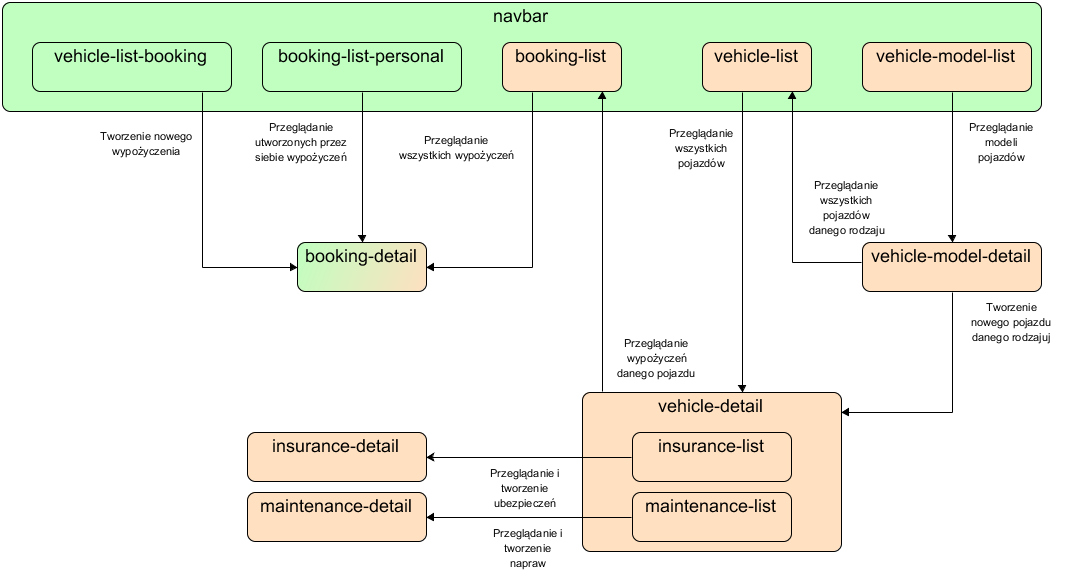
\includegraphics[width=\textwidth]{images/angular_views.png}
		\caption{Widoki interfejsu użytkownika.}
		\small 
		Widoki zielone dostępne są dla każdego użytkownika; widoki pomarańczowe wyłącznie dla użytkownika o odpowiednich uprawnieniach. Widok \textit{booking-detail} jest specjalnym przypadkiem oferującym różne możliwości w zależności od uprawnień użytkownika.
	\end{figure}

	\section{Walidacja danych}
	Dane wprowadzane przez użytkownika są sprawdzane pod kątem poprawności. W przypadku pól tekstowych walidacja najczęściej weryfikuje obecność jakiegokolwiek tekstu; pola, które powinny zawierać liczby, są weryfikowane przy użyciu wyrażeń regularnych.
	
	\lstinputlisting[frame=single,caption=Przykładowy walidator używający wyrażenia regularnego.]{source/validator.js}
	
	W przypadku wykrycia błędnych danych, pod polem zawierającym niepoprawne dane pojawia się opis błędu oraz przycisk zatwierdzający zmiany zostaje zablokowany.
	\begin{figure}[H]
		\centering
		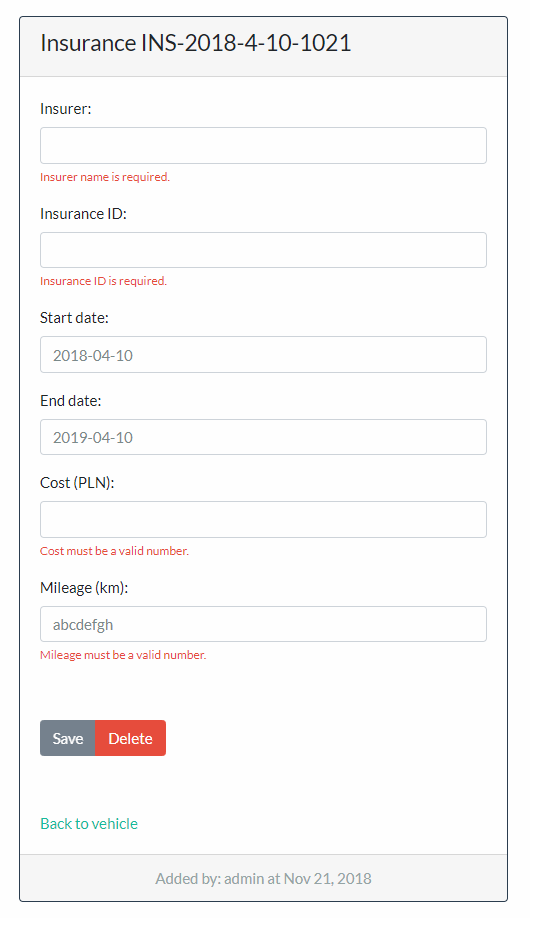
\includegraphics[scale=0.7]{images/insurance_validation_errors.png}
		\caption{Widok z polami zawierającymi błędne wartości.}
	\end{figure}

	\newpage
	\section{Stopka audytowa}
	Każdy widok szczegółowy korzysta z komponentu \textit{AuditFooter} wyświetlającego nazwę użytkownika, który utworzył/modyfikował obiekt oraz datę kiedy akcja została wykonana.
	
	\begin{figure}[H]
		\centering
		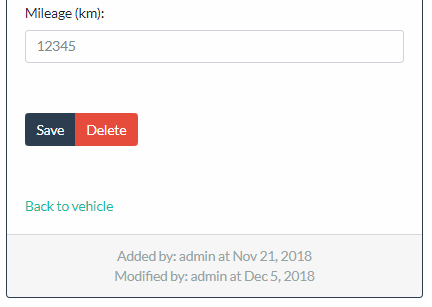
\includegraphics[scale=0.5]{images/insurance_footer.png}
		\caption{Stopka audytowa.}
	\end{figure}

	\section{Dialogi}
	Każda akcja która niesie za sobą znaczne (np. akceptacja rezerwacji) lub nieodwracalne (np. usunięcie obiektu) musi zostać zatwierdzona przez użytkownika w dialogu który pojawia się po naciśnięciu przycisku zapisu/usuwania.
	
	\begin{figure}[H]
		\centering
		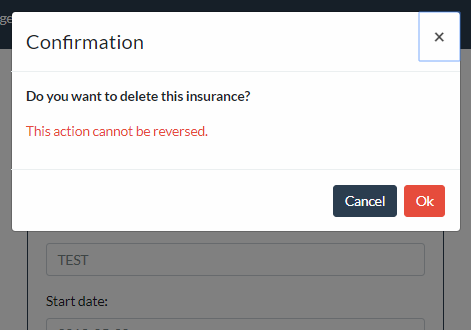
\includegraphics[scale=0.7]{images/insurance_confirmation.png}
		\caption{Przykładowy dialog.}
	\end{figure}
	
	%\section{Konteneryzacja}
	%----------------------------------------------------------------------------------------
	%	SECTION 6
	%----------------------------------------------------------------------------------------
	%\newpage
	%\chapter{Implementacja}
	
	%----------------------------------------------------------------------------------------
	%	SECTION 7
	%----------------------------------------------------------------------------------------
	\newpage
	\chapter{Testy}
	\section{Testy jednostkowe}
	System był testowany przy użyciu testów jednostkowych korzystających z biblioteki \textit{XUnit} oraz napisanych w schludny, zgodny z często stosowaną w języku C\# konwencją \textit{AAA} sposób, bazujący na podziale testu na trzy sekcje:
	\begin{enumerate}
		\item Przygotuj (\textit{Arrange}): przygotowanie niezbędnych zmiennych
		\item Działaj (\textit{Act}): wywołanie metod, które mają być testowane 
		\item Sprawdź (\textit{Assert}): sprawdzenie wyniku 
	\end{enumerate}
	W testach klas wymagających wstrzykiwania zależności wykorzystano bibliotekę \textit{Moq} do tworzenia atrap obiektów.
	
	Przetestowane zostały m. in. kluczowe funkcjonalności kontrolerów oraz metody rozszerzeń.
	
	\lstinputlisting[language=C,frame=single,caption=Test jednostkowy metody rozszerzeń.]{source/tests-unit.cs}
	\newpage
	\lstinputlisting[language=C,frame=single,caption=Test kontrolera korzystający z \textit{Moq}.]{source/tests-integration.cs}
	
	\newpage
	\section{Testy systemowe}
	Najczęściej stosowanym rodzajem testów były testy systemowe przy użyciu narzędzia \textit{Postman} pozwalającego na wygodne tworzenie i wysyłanie skomplikowanych żądań \textit{HTTP}. \textit{Postman} pozwala również na zapisywanie oraz organizowanie żądań co znacznie przyśpiesza proces testowania.
	\begin{figure}[H]
		\centering
		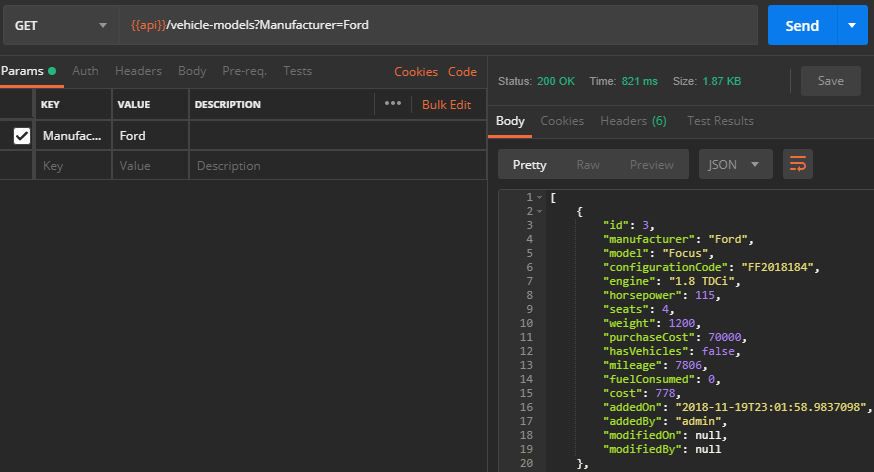
\includegraphics[width=\textwidth]{images/tests_postman.png}
		\caption{Interfejs programu Postman.}
	\end{figure}
	\section{Testy dymne}
	Testy dymne (\textit{ang. smoke test}) były użyte w końcowej fazie projektu; polegały na wcieleniu się w rolę użytkownika i przechodzeniu najczęściej używanych ścieżek (np. tworzeniu rezerwacji). Testy tego typu pozwalają szybko zweryfikować czy kluczowa funkcjonalność systemu działa bezproblemowo.
	
	%----------------------------------------------------------------------------------------
	%	SECTION 8
	%----------------------------------------------------------------------------------------
	\newpage
	\chapter{Podsumowanie}
	\section{Wnioski}
	Celem pracy było utworzenie systemu pozwalającego na kontrolę dostępu do pojazdów oraz śledzeniu ich stanu; cel ten został spełniony. System został napisany w sposób zgodny ze standardami, co pozwala na łatwiejsze utrzymanie (w tym dalszą rozbudowę). Zastosowanie nowoczesnych technologii takich jak framework \textit{ASP.NET Core 2.1} pozwala na łatwe rozwijanie aplikacji przy użyciu języka \textit{C\#}, dodatkowo oferując wiele zalet takich jak multiplatformowość i zwiększoną wydajność względem tradycyjnego \textit{ASP.NET Framework}. Użycie aplikacji webowej jako interfejsu użytkownika pozwala na dostęp do systemu bez potrzeby instalacji aplikacji klienckiej. Aplikacja webowa eliminuje również problemy takie jak aktualizacje do nowych wersji i zmniejsza koszt utrzymania całego systemu.
	
	\section{Możliwości rozwoju}
	System może być rozwinięty na wiele sposobów; kilka z nich:
	\begin{itemize}
		\item automatyczna generacja raportów o kosztach (np. co miesiąc) oraz wprowadzenie serwisu wysyłającego raport e-mailem do użytkowników,
		\item wyświetlanie statystyk w formie graficznej w interfejsie użytkownika,
		\item przystosowanie aplikacji to użycia na urządzeniach mobilnych,
		\item udostępnienie interfejsu programistycznego innym systemom — przykładowo system zbierający koszty generowane przez dany dział w firmie mógłby sprawdzać wydatki pracownika wiążące się z rezerwowaniem pojazdów,
		\item konteneryzacja aplikacji,
		\item przechowywanie pełnej historii edycji oraz generowanie raportów audytowych w formacie zgodnym z \textit{Microsoft Excel}.
	\end{itemize}
	
	
	%----------------------------------------------------------------------------------------
	%	SECTION OLD
	%----------------------------------------------------------------------------------------
	
	%----------------------------------------------------------------------------------------
	%	SECTION OLD
	%----------------------------------------------------------------------------------------
	
	%\chapter{Projekt systemu}
	%System można podzielić na dwa elementy — interfejs użytkownika (\textit{UI}) oraz interfejs programistyczny (\textit{API}). Komunikacja między interfejsami odbywa się według protokołu \textit{HTTP}; dane przesyłane są w formacie \textit{JSON}.
	%
	%Dostęp do systemu został zabezpieczony przy użyciu standardu \textit{JSON Web Token (JWT)}. Autoryzacja \textit{JWT} działa w następujący sposób:
	%\begin{enumerate}
	%	\item Użytkownik loguje się przez interfejs użytkownika, podając nazwę użytkownika oraz hasło
	%	\item Interfejs programistyczny weryfikuje dane logowania
	%	\item W przypadku prawidłowego hasła utworzony zostaje token \textit{JWT} zawierający:
	%		\subitem Informacje o wydającym token
	%		\subitem Informacje o użytkowniku: jego identyfikator (nazwa użytkownika) oraz role
	%	\item Utworzony token zostaje zaszyfrowany (uniemożliwiając jego sfałszowanie)i przesłany 		
	%	\item Odebrany token zostaje umieszczony w pamięci przeglądarki internetowej użytkownika
	%\end{enumerate}
	%Interfejs programistyczny weryfikuje poprawność tokena dla każdego żądania \textit{HTTP} z wyjątkiem tych związanych z procesem autoryzacji użytkownika; jeżeli token jest niepoprawny lub zbyt stary (wydany więcej niż 2 godziny przed weryfikacją), żądanie jest odrzucone.
	%
	%
	%[[ tutaj dodam zdjęcie tokenu z systemu przed i po szyfrowaniu ]]
	
	%----------------------------------------------------------------------------------------
	%	APPENDIX
	%----------------------------------------------------------------------------------------
	%\appendix
	%\chapter{Donec cursus nulla vitae pede}
	%Donec cursus nulla vitae pede. Etiam quam pede, aliquet ut, pellentesque sed, sagittis non, est. Quisque egestas malesuada risus. Maecenas ultricies libero a quam. Nullam feugiat arcu. Class aptent taciti sociosqu ad litora torquent per conubia nostra, per inceptos hymenaeos. In interdum, risus ut gravida sollicitudin, leo sapien commodo dui, non consectetuer nisl nunc ac massa. Mauris a orci in eros venenatis euismod. Curabitur orci. Quisque pharetra, dui sed dignissim hendrerit, nibh ante malesuada eros, sed tincidunt magna lorem a tellus. Aliquam erat volutpat. Aenean pulvinar, metus et mattis dictum, massa lacus semper purus, quis vehicula augue mi et leo. Ut eu ipsum. Sed dictum dapibus nisi. Cras mattis.
	
	%----------------------------------------------------------------------------------------
	%	END
	%----------------------------------------------------------------------------------------
	\addcontentsline{toc}{chapter}{Literatura}
	\bibliography{bibliography}
	
	\newpage 
	
	\begin{appendices}
		
		\chapter{Instrukcja użytkownika}
		\section{Ekran logowania}
		Jedyny widok dostępny dla niezalogowanego użytkownika. Aplikacja uniemożliwia dostęp do wszystkich innych widoków osobom niezalogowanym; przy ręcznej zmianie adresu w przeglądarce nieupoważniony użytkownik zostanie przekierowany do tego widoku.
		\begin{figure}[H]
			\centering
			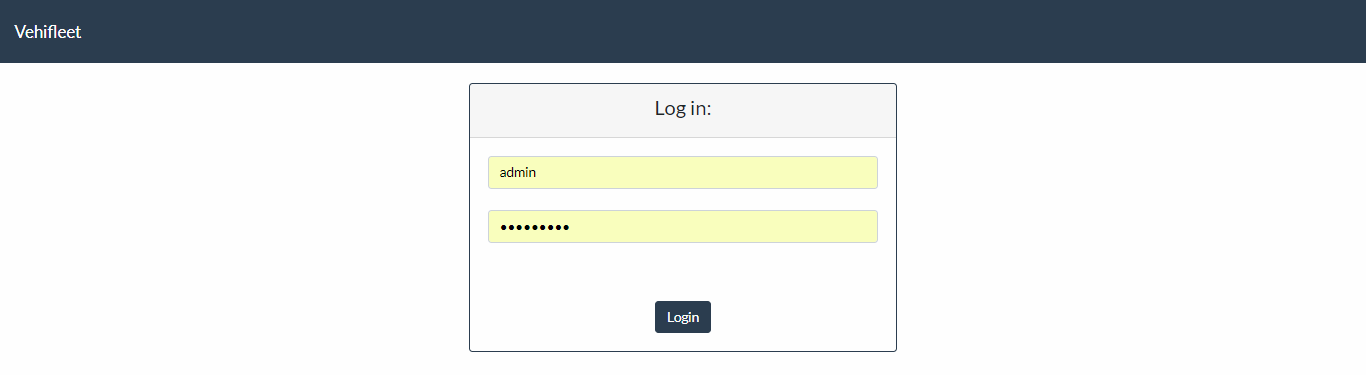
\includegraphics[width=\textwidth]{images/views/dashboard-login.png}
			\caption{Widok logowania (dashboard-login).} 		
		\end{figure}
		
		\section{Ekran wylogowywania}
		Podstawowy widok zalogowanego użytkownika z informacjami o użytkowniku i możliwością wylogowania się.
		\begin{figure}[H]
			\centering			
			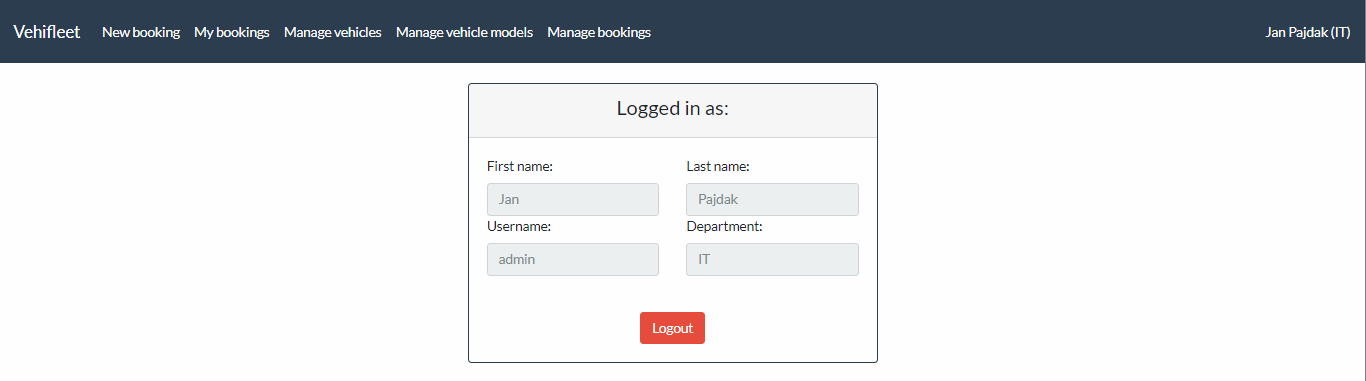
\includegraphics[width=\textwidth]{images/views/dashboard-logout.png}
			\caption{Widok zalogowanego użytkownika (dashboard-user-details).} 
		\end{figure}
		
		\section{Dostępne pojazdy}
		Widok pozwalający na przeglądanie oraz rezerwowanie dostępnych pojazdów, otwierana z poziomu paska nawigacyjnego, za pomocą przycisku (\textit{Vehicle Booking}). Lista pojazdów może być dodatkowo filtrowana. Po kliknięciu na jakikolwiek pojazd, jego dokładne informacje zostają wczytane i wyświetlone w oknie po prawej stronie; użytkownik może utworzyć nową rezerwację używając przycisku \textit{Book}. 
		\begin{figure}[H]
			\centering
			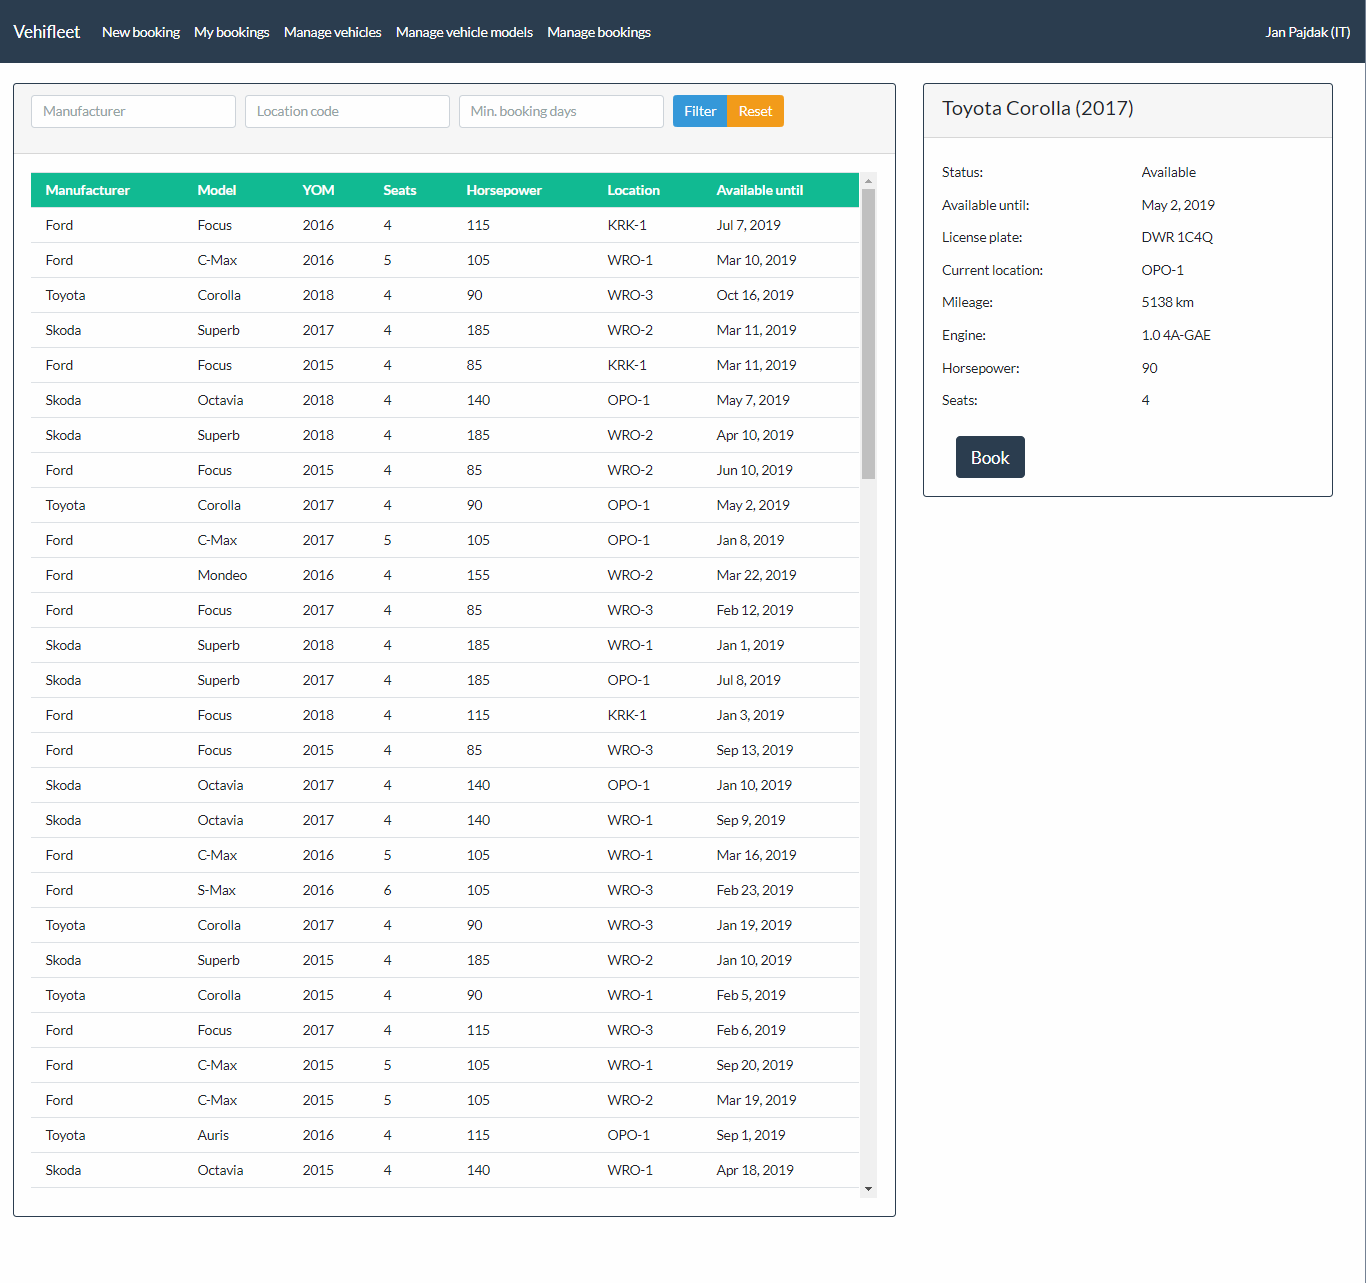
\includegraphics[width=\textwidth]{images/views/vehicle-booking-2.png}
			\caption{Widok listy dostępnych pojazdów (vehicle-list-booking).}
		\end{figure}
		
		\newpage
		\section{Historia rezerwacji}
		Widok (pozycja \textit{My bookings} na pasku nawigacyjnym) zawiera rezerwacje utworzone tylko i wyłącznie przez zalogowanego użytkownika; użytkownik bez praw kierownika nie jest w stanie przeglądać cudzych rezerwacji. Kliknięcie w rekord otwiera szczegółowy widok rezerwacji.
		\begin{figure}[H]
			\centering
			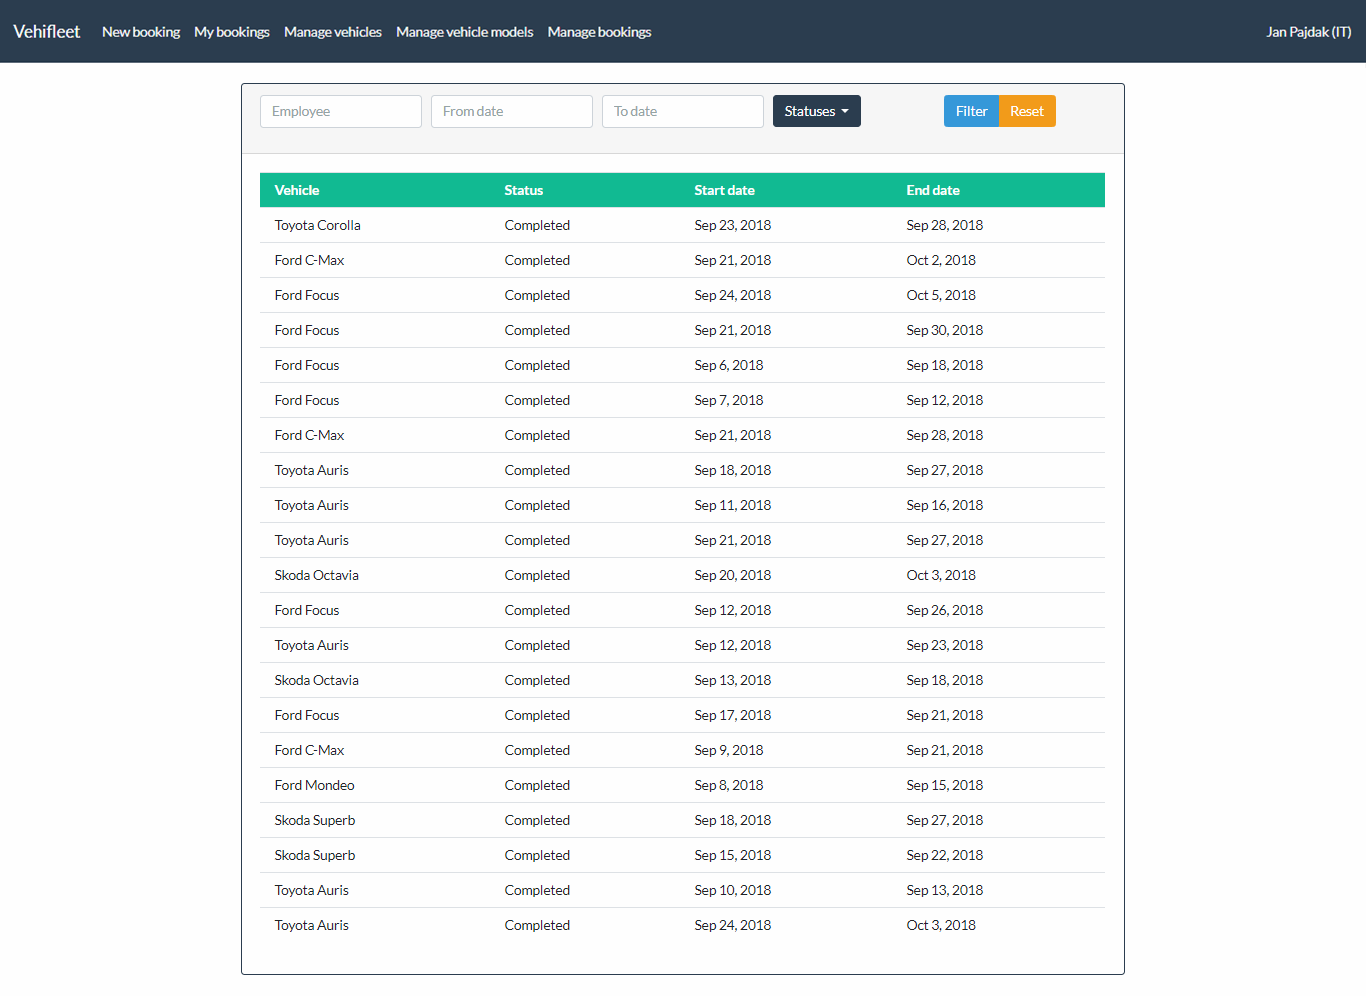
\includegraphics[width=\textwidth]{images/views/booking-list-manage.png}
			\caption{Widok listy historii rezerwacji (booking-personal).}	
		\end{figure}
		
		\newpage
		\section{Szczegóły rezerwacji}
		W tym widoku można zarówno utworzyć nowe rezerwację, jak i edytować już istniejące.
		\begin{figure}[H]
			\centering
			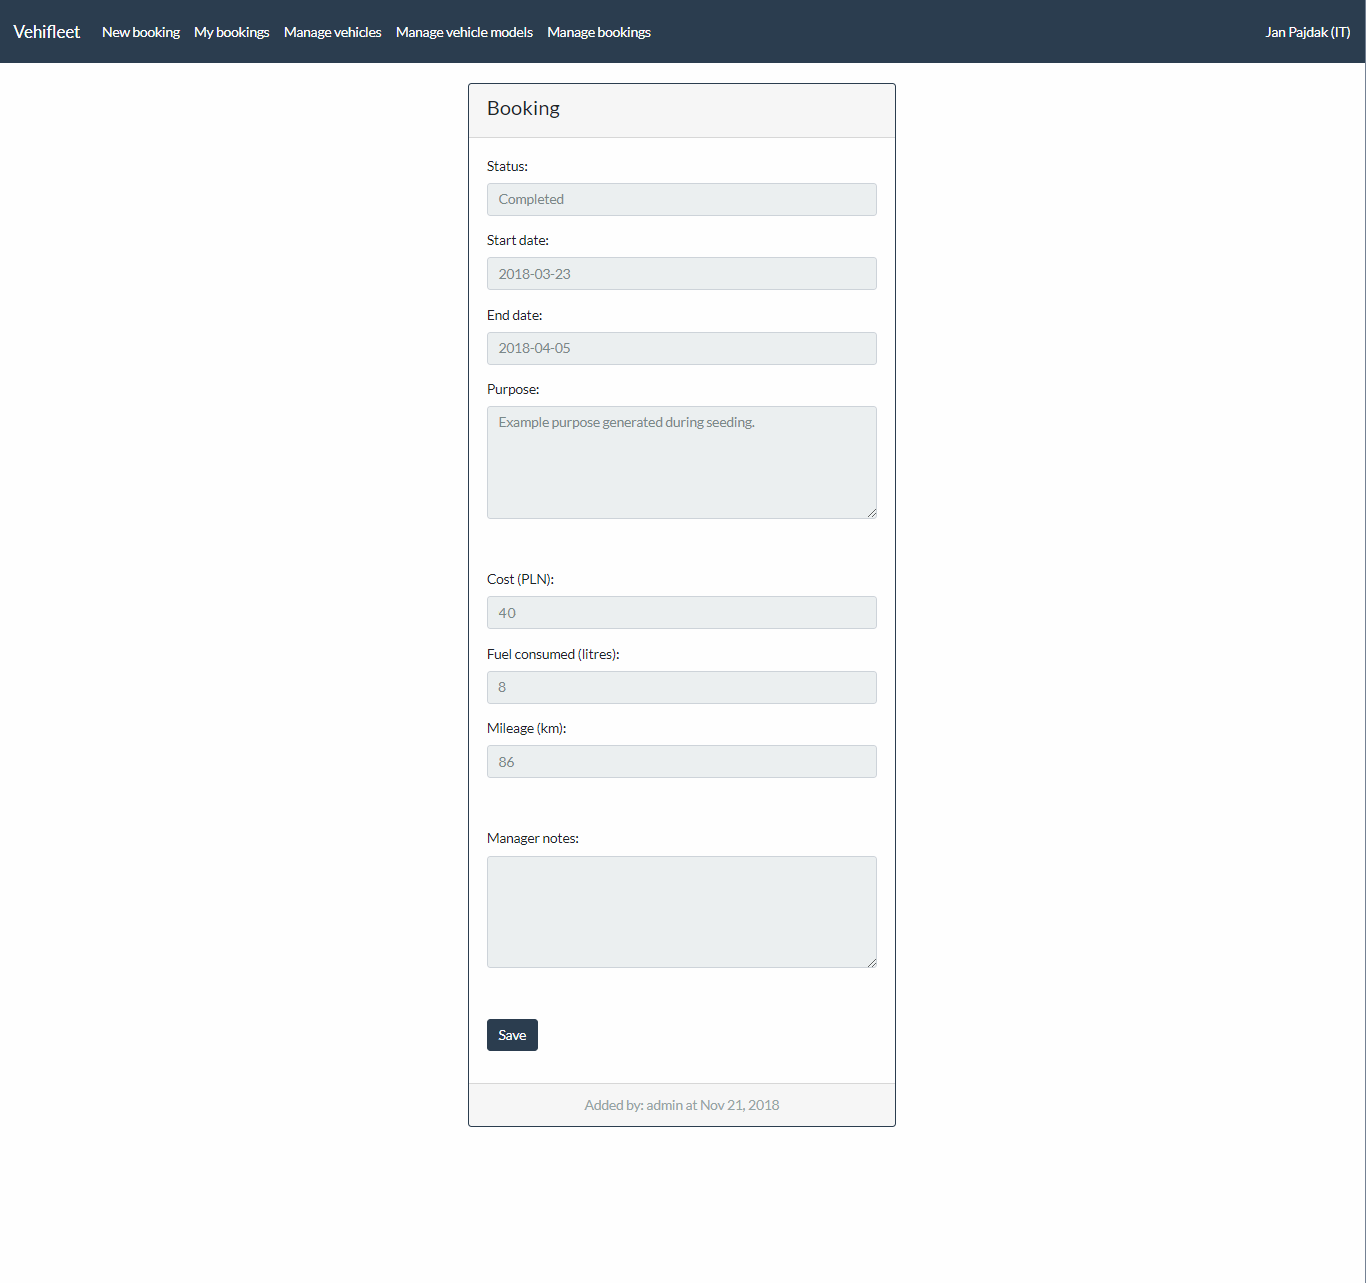
\includegraphics[width=\textwidth]{images/views/booking-detail.png}
			\caption{Widok szczegółowy rezerwacji (booking-details).} 		
		\end{figure}
		
		\newpage	
		\subsection{Szczegóły rezerwacji w trybie kierownika}
		Jeżeli zalogowanym użytkownikiem jest kierownik, wyświetlony zostaje dodatkowy panel z informacjami o użytkowniku który utworzył rezerwację. 		
		\begin{figure}[H]
			\centering
			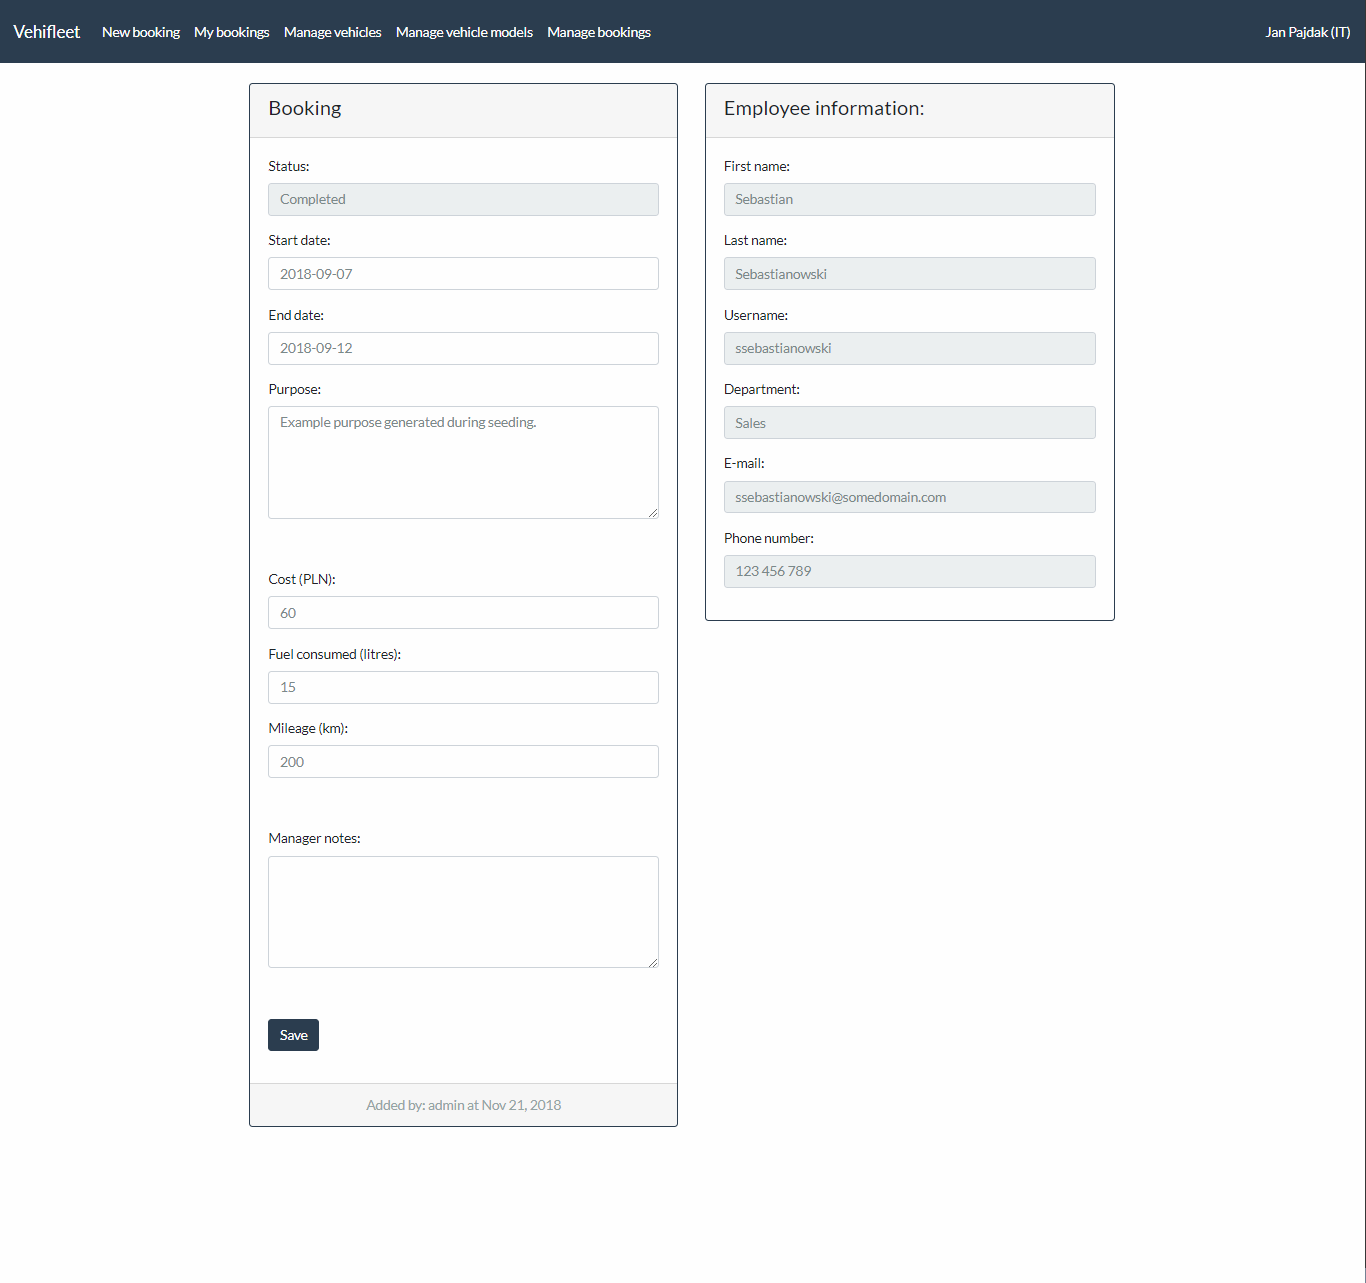
\includegraphics[width=\textwidth]{images/views/booking-detail-manager.png}
			\caption{Widok szczegółowy rezerwacji w trybie kierownika (booking-details).}		
		\end{figure}
		
		\newpage
		\section{Wszystkie pojazdy}
		Widok dostępny wyłącznie dla kierowników; jeżeli zalogowany użytkownik posiada odpowiednie uprawnienia, może przejść do tego widoku za pomocą przycisku \textit{Manage vehicles} na pasku nawigacyjnym.
		
		Widok pozwala na przeglądanie wszystkich pojazdów. Lista może być filtrowana po numerze karoserii, kodzie obecnej lokalizacji oraz statusie. Kliknięcie na pojazd otwiera jego widok szczegółowy.
		\begin{figure}[H]
			\centering
			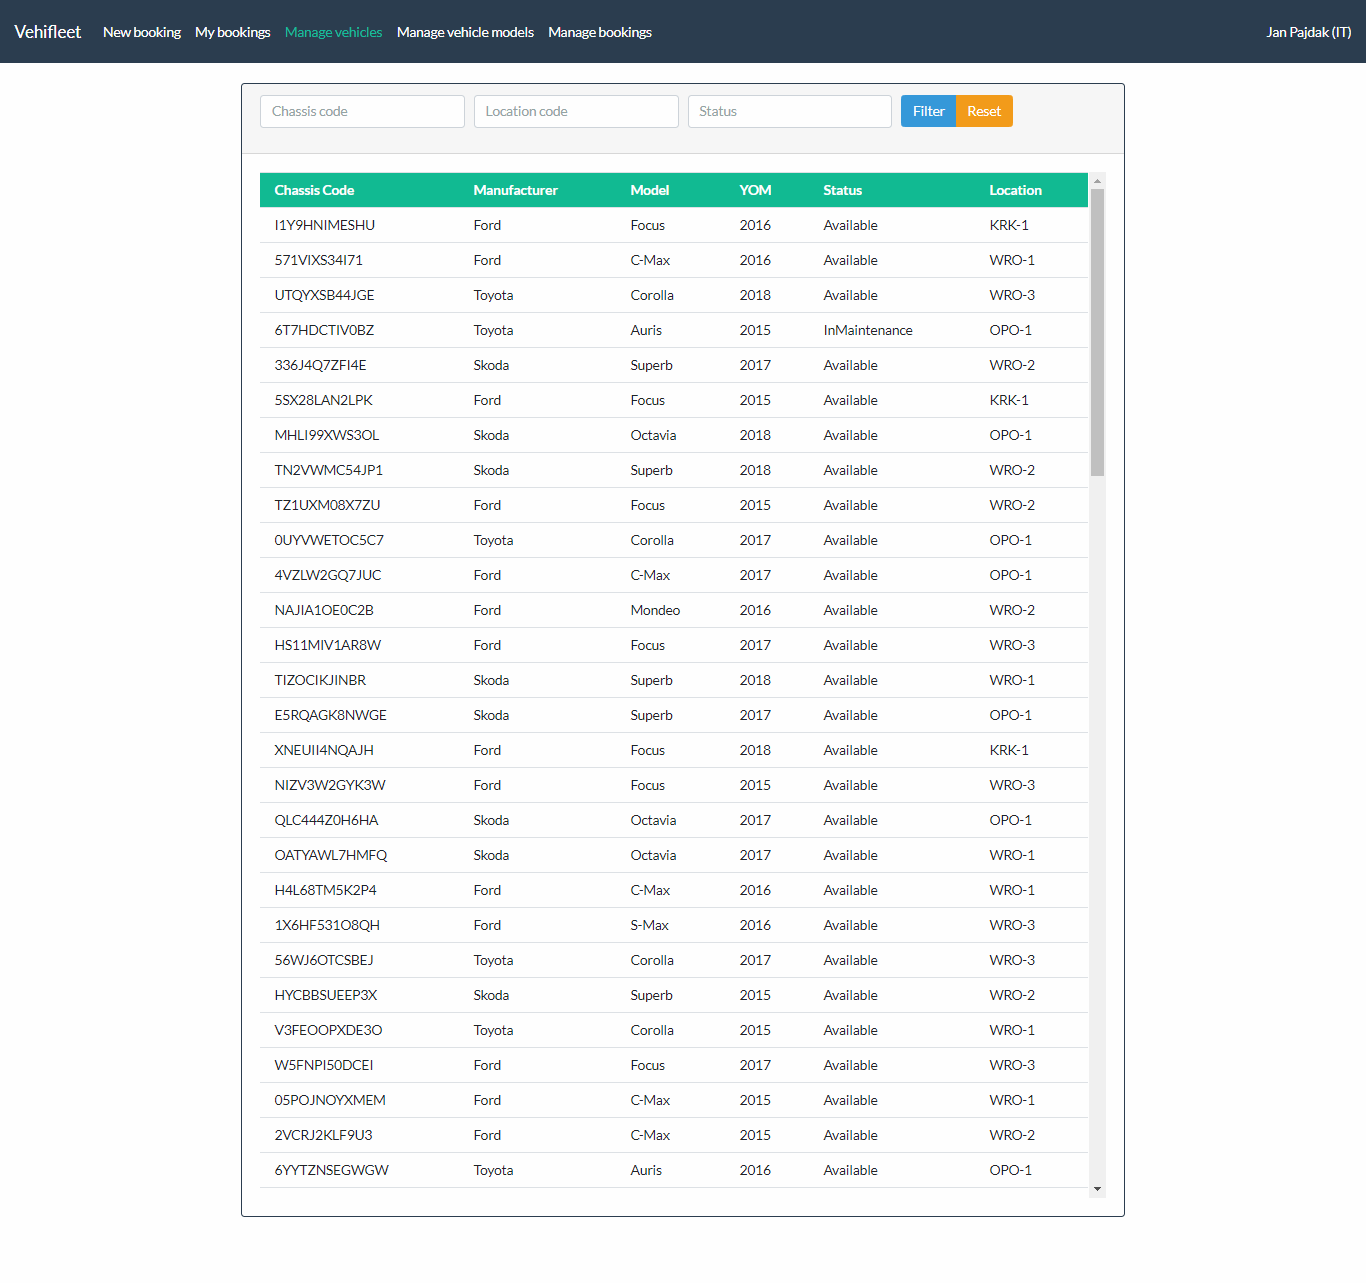
\includegraphics[width=\textwidth]{images/views/vehicle-list.png}
			\caption{Widok listy pojazdów (vehicle-list).}
		\end{figure}
		
		\newpage
		\section{Szczegóły pojazdu}	
		\begin{figure}[H]

			Widok zawierający wszystkie informacje na temat pojazdu wraz z listą ubezpieczeń i napraw, które mogą być dodawane lub edytowane. Przejście do widoków szczegółowych ubezpieczeń/napraw odbywa się przez kliknięcie na odpowiedni wiersz w liście; wprowadzanie nowych informacji odbywa się odpowiednio przy użyciu przycisków \textit{New Insurance} i \textit{New Maintenance} Użytkownik może wyświetlić wszystkie rezerwacje danego pojazdu lub jego dokładną specyfikacje techniczną po kliknięciu na odpowiedni odnośnik na dole okna.
			
			Pojazd nie może być edytowany jeżeli jest obecnie zarezerwowany.
			\centering
			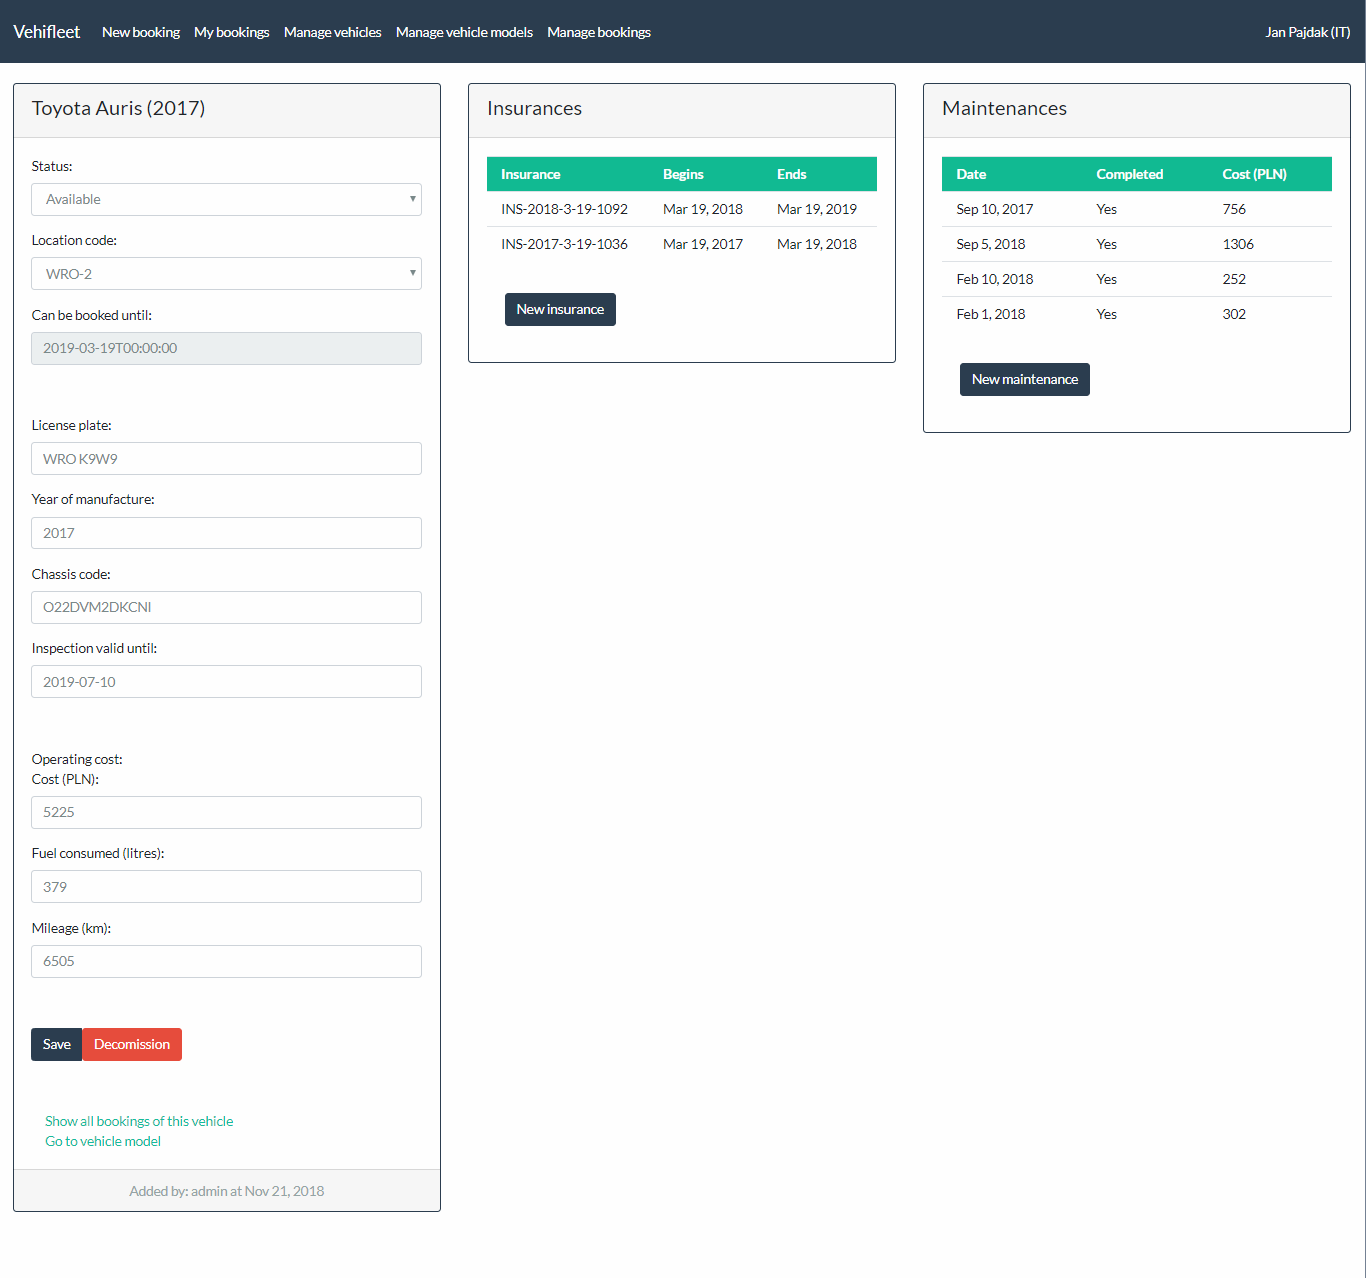
\includegraphics[width=\textwidth]{images/views/vehicle-detail.png}
			\caption{Widok szczegółowy pojazdu (vehicle-details).}		
		\end{figure}
		
		\newpage
		\section{Szczegóły ubezpieczenia}
		Widok pozwalający na utworzenie lub modyfikację ubezpieczenia.
		\begin{figure}[H]
			\centering
			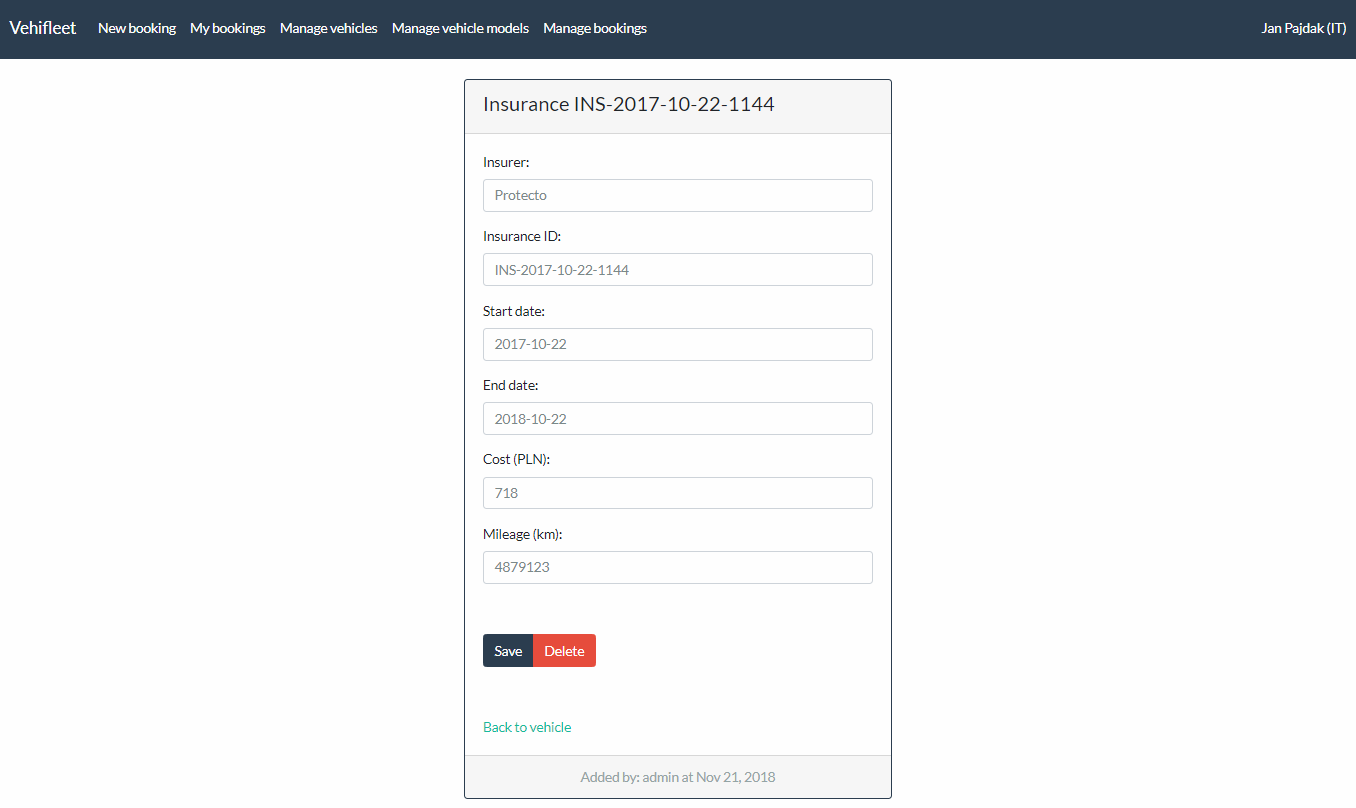
\includegraphics[scale=0.32]{images/views/insurance-detail.png}
			\caption{Widok szczegółowy ubezpieczenia (insurance-details).}		
		\end{figure}
		
		\section{Szczegóły naprawy}
		Widok pozwalający na utworzenie lub modyfikację zdarzenia serwisowego.
		\begin{figure}[H]
			\centering
			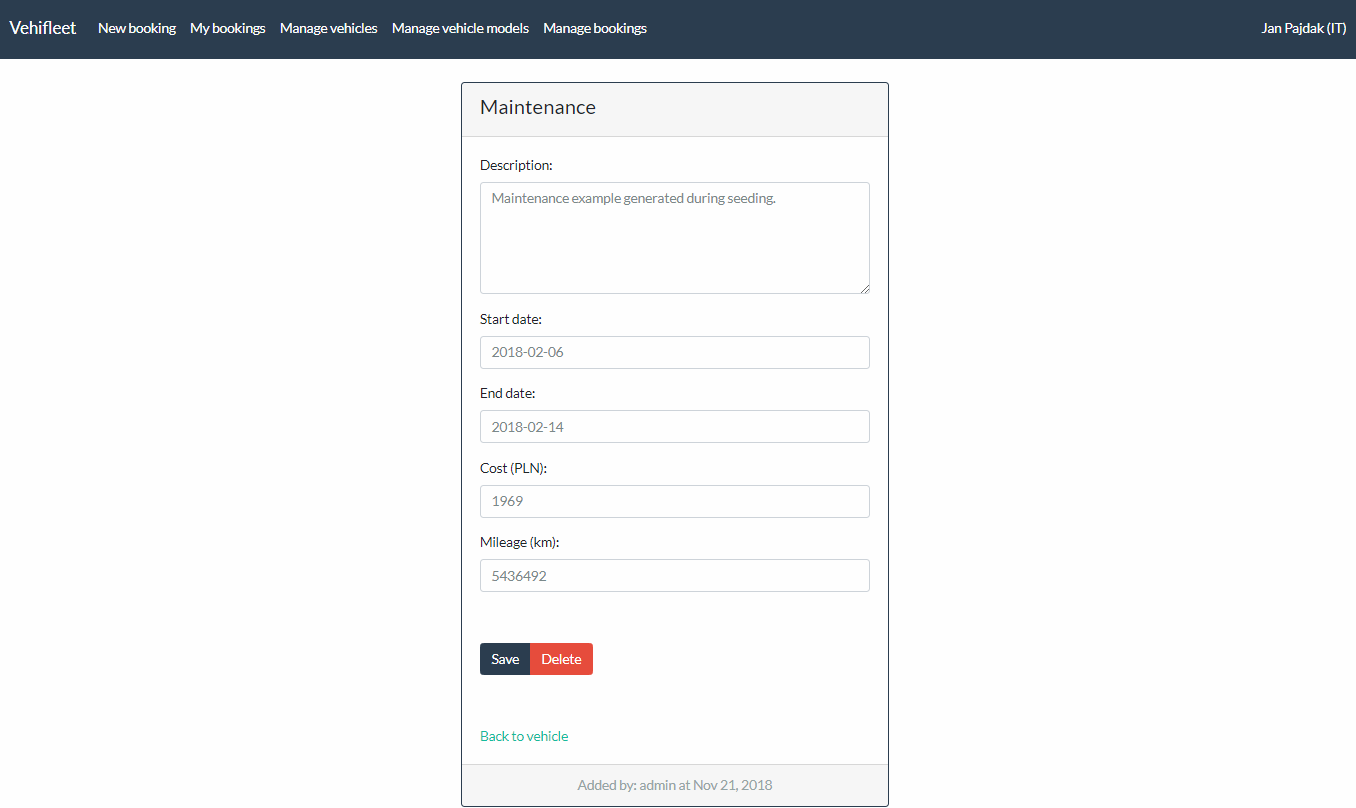
\includegraphics[scale=0.32]{images/views/maintenance-detail.png}
			\caption{Widok szczegółowy naprawy (maintenance-details).}
		\end{figure}
		
		\newpage	
		\section{Wszystkie modele pojazdów}	
		Widok dostępny wyłącznie dla kierowników; jeżeli zalogowany użytkownik posiada odpowiednie uprawnienia, może przejść do tego widoku za pomocą przycisku \textit{Manage vehicle models} na pasku nawigacyjnym.
		
		Widok zawiera listę modeli pojazdów; lista może być filtrowana po nazwie producenta. Kliknięcie na wiersz przechodzi do widoku szczegółowego danego pojazdu.
		
		Pod listą znajduje się przycisk umożliwiający wprowadzenie nowego modelu.
		\begin{figure}[H]
			\centering
			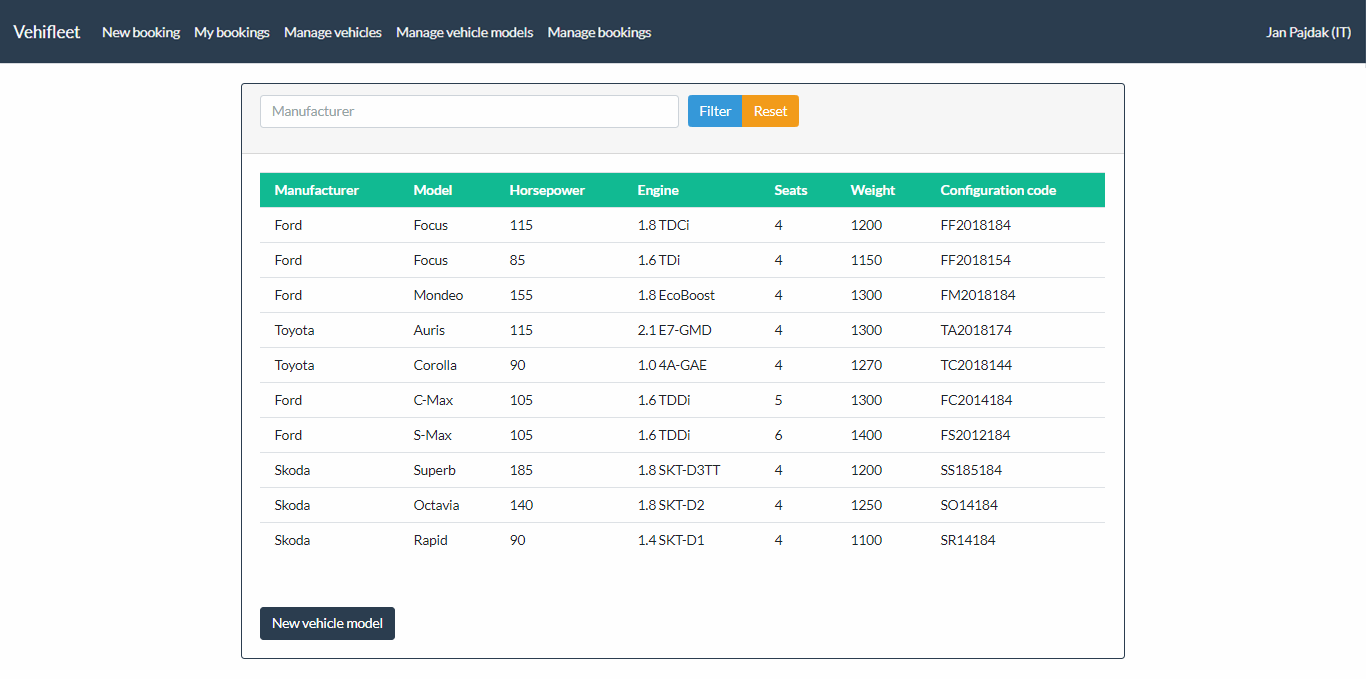
\includegraphics[width=\textwidth]{images/views/vehicle-model-list.png}
			\caption{Widok listy modeli pojazdów (vehicle-model-list).}
		\end{figure}
		
		\newpage
		\section{Szczegóły modelu pojazdu}
		Widok pozwala na dodawanie oraz edycje modeli pojazdów. Za pomocą odnośników na dole strony można wyszukać wszystkie pojazdy danego rodzaju oraz wprowadzić nowy egzemplarz.
		\begin{figure}[H]
			\centering
			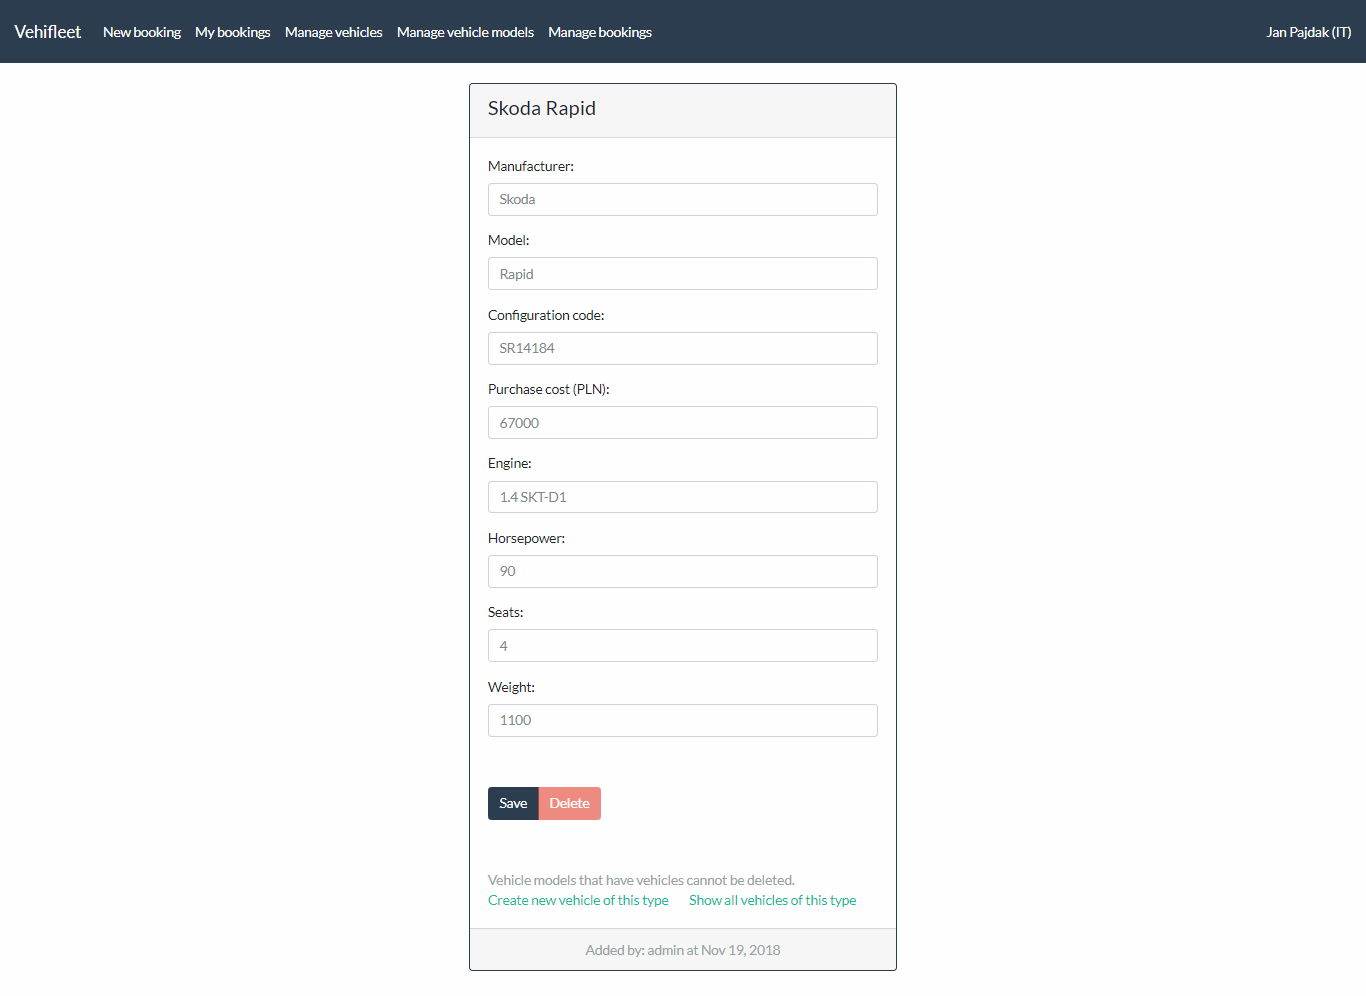
\includegraphics[width=\textwidth]{images/views/vehicle-model-detail.png}
			\caption{Widok szczegółowy modelu pojazdu (vehicle-model-details).}
		\end{figure}
	\end{appendices}
\end{document}

